\documentclass{aghdpl}
% \documentclass{aghdpl}               % przy kompilacji programem latex
% \documentclass[pdflatex,en]{aghdpl}  % praca w języku angielskim
\usepackage[polish]{babel}
\usepackage[utf8]{inputenc}

% dodatkowe pakiety
\usepackage{verbatim}
\usepackage{wrapfig}
\usepackage{listings}
\usepackage{hyperref}
\usepackage{userstory}
\usepackage{packed_enum}
\usepackage{packed_item}
\usepackage{layouts}
\usepackage{capt-of}
\usepackage{graphicx}
\usepackage{caption}
\usepackage{subcaption}
\usepackage{epstopdf}

% ustawienie kolorów
\hypersetup{
    colorlinks,
    citecolor=black,
    filecolor=black,
    linkcolor=black,
    urlcolor=black
}
% kilka swoich komend do odnośników
% z w rozdziale
\newcommand\namedref[1]{w~rozdziale \ref{#1}~\nameref{#1}}
% bez w rozdziale
\newcommand\namedrefw[1]{\ref{#1}~\nameref{#1}}

% w itemize, chcemy kropki, a nie pauzy
\renewcommand{\labelitemi}{$\bullet$}

\usepackage{color}
\definecolor{dkgreen}{rgb}{0,0.6,0}
\definecolor{gray}{rgb}{0.5,0.5,0.5}
\definecolor{mauve}{rgb}{0.58,0,0.82}
\lstset{
  literate={ą}{{\k{a}}}1
           {ć}{{\'c}}1
           {ę}{{\k{e}}}1
           {ó}{{\'o}}1
           {ń}{{\'n}}1
           {ł}{{\l{}}}1
           {ś}{{\'s}}1
           {ź}{{\'z}}1
           {ż}{{\.z}}1
           {Ą}{{\k{A}}}1
           {Ć}{{\'C}}1
           {Ę}{{\k{E}}}1
           {Ó}{{\'O}}1
           {Ń}{{\'N}}1
           {Ł}{{\L{}}}1
           {Ś}{{\'S}}1
           {Ź}{{\'Z}}1
           {Ż}{{\.Z}}1,
    language=[AlLaTeX]TeX,
    basicstyle=\footnotesize,
    numbers=left,
    numberstyle=\tiny\color{gray},
    stepnumber=2,
    frame=false,
    breaklines=true,
    tabsize=4,
    showspaces=false,
    showstringspaces=false,
    showtabs=false,
    caption=\lstname,
    commentstyle=\color{dkgreen},
    stringstyle=\color{mauve}
}
%---------------------------------------------------------------------------

\author{Leszek Piątek}
\shortauthor{L. Piątek}

\titlePL{Społecznościowy, internetowy system monitoringu}
\titleEN{Social, Internet monitoring system}

\shorttitlePL{Społecznościowy, internetowy system monitoringu} % skrócona wersja tytułu jeśli jest bardzo długi
\shorttitleEN{Social, Internet monitoring system}

\thesistypePL{Praca magisterska}
\thesistypeEN{Master of Science Thesis}

\supervisorPL{dr inż. Sebastian Ernst}
\supervisorEN{Sebastian Ernst PhD}

\date{2012}

\departmentPL{Katedra Informatyki Stosowanej}
\departmentEN{Department of Applied Computer Science}

\facultyPL{Wydział Elektrotechniki, Automatyki, Informatyki i Elektroniki}
\facultyEN{Faculty of Electrical Engineering, Automatics, Computer Science and Electronics}

\acknowledgements{Serdecznie dziękuję promotorowi dr~inż.~Sebastianowi~Ernstowi za dystans, wyrozumiałość i cierpliwość.\footnote{Rozwinięcie podziękowań znajduje się w dodatku \namedrefw{cha:dodatekB}.}}

\setlength{\cftsecnumwidth}{10mm}

%---------------------------------------------------------------------------

% Moje zmienne
\def\todo{Do uzupełnienia/dokończenia później...}
\def\toworkon#1{Do dopracowania: \textit{#1}}

% Struktura dokumentu
\begin{document}

\hypersetup{pageanchor=false}
\titlepages
\hypersetup{pageanchor=true}
\urlstyle{same}

\tableofcontents
\clearpage

\chapter{Wprowadzenie}
\label{cha:wprowadzenie}

W ostatnich latach można zauważyć gwałtowny rozwój rozwój infrastruktury i technologii sieciowych. Coraz więcej gospodarstw domowych dołącza się do ,,chmury informacyjnej'' jaką jest Internet. Komputery bez dostępu do sieci powoli stają się po prostu bezużyteczne. Internet dzięki Wi-Fi oraz technologiom telefonii komórkowej takich jak HSPA lub jej następcy LTE staje się medium bezprzewodowym, dostępnym wszędzie tam gdzie istnieje zasięg sieci komórkowej.

Wszechobecność i dostępność ,,wielkiej pajęczyny'' powoduje, że coraz częściej korzysta się z niej nie tylko za pomocą komputerów czy laptopów. Nowe ,,gadżety'' takie jak tablety, smartphone'y czy netbooki stają się nowym interfejsem pomiędzy siecią, a użytkownikiem. Szacuje się, że do roku 2015 większość użytkowników Internetu będzie korzystała właśnie z takich urządzeń mobilnych. Wtedy również, 40\% światowej populacji (2,7 miliarda osób) będzie już korzystała z dobrodziejstw dostępu do ,,natychmiastowej informacji''. \footnote{Dane w oparciu o  artykuł \cite{Kim11}}

Zwiększenie szybkości dostępu do Internetu umożliwiło stworzenie technologii pozwalających na transmisję strumieniową danych audio/wideo. Takie serwisy jak YouTube, Vimeo czy MetaCafe już od 2005 roku umożliwiają użytkownikom wysyłanie i udostępnianie swoich nagrań online. Niestety żaden z tych serwisów nie umożliwiał udostępniania strumienia danych wideo w czasie rzeczywistym. Dopiero w 2007 roku powstał Bambuser oraz Qik. W tym roku, dosłownie parę miesięcy temu firma Google połączyła usługę YouTube z Google+ Hangouts umożliwiając równoczesne nadawanie ,,na żywo''. Wszystkie serwisy te jak i technologie, które wdrożyły, pozwalają dzielić się strumieniem audio/video -- wykorzystując do tego jedynie telefon komórkowy lub kamerę podłączoną do komputera.

Naturalną koleją rzeczy wydaje się wykorzystanie Internetu celem stworzenia gigantycznego systemu monitoringu. Można sobie wyobrazić system do którego podłączono istniejącą infrastrukturę kamer CCTV i udostępniono ich strumień video online, tak aby każdy obywatel mógł monitorować to co się dzieje w jego okolicy. System można by było rozszerzyć o kamery podłączane przez użytkowników lub ich najnowocześniejsze ,,gadżety'' czyli tablety czy smartphone'y. Tak właśnie autor niniejszej pracy wyobraża sobie ,,Społecznościowy, internetowy system monitoringu''.

\newpage
%---------------------------------------------------------------------------

\section{Cele pracy}
\label{sec:celePracy}

Głównym celem pracy, a co za tym idzie i najbardziej czasochłonnym celem pracy jest implementacja ograniczonego prototypu systemu określanego mianem ,,Społecznościowy, internetowy system monitoringu''.

Dodatkowym celem, bo koniecznym do realizacji głównego, jest stworzenie specyfikacji oraz analizy wymagań systemu określonego jako ,,Społecznościowy, internetowy system monitoringu''. Na każdym etapie przygotowywania projektu, chciano wykorzystać jak najwięcej metodyk i technologii ,,zwinnych''. Dlatego też bazując na pracy starszych kolegów (\cite{JakMich06}), jak i doświadczeniu w zwinnym specyfikowaniu systemu doktorantów (\cite{Mad09}), podpierając się literaturą fachową (\cite{Bec99}) autor chce zaproponować własną ,,zwinną specyfikację i analizę wymagań''. W szczególności pokazać jej zalety oraz wady względem podejścia konwencjonalnego. Uwypuklić przypadki, w których metodyki zwinne nie są dobrym rozwiązaniem.

\section{Zawartość pracy}
\label{sec:zawartoscPracy}

W pierwszym rozdziale pracy opisano teorię związaną ze ,,zwinną'' metodyką tworzenia oprogramowania. Umieszczono jej wady, zalety oraz wyszczególniono kiedy nie należy stosować metodyk zwinnych. Tutaj znalazło się również miejsce na opisanie idealnego cyklu życia idealnego ,,zwinnego'' projektu oraz autorską propozycję przeprowadzania akwizycji i analizy wymagań takiego przedsięwzięcia.

Kolejny rozdział pracy poświęcony jest akwizycji i analizie wymagań tytułowego ,,Społecznościowego systemu monitoringu''. W tej części pracy znajdują się więc takie elementu jak karty wymagań, ekrany, wstępna architektura systemu czy opis technologii proponowanych do zastosowania. Przy realizacji ww. elementów wykorzystano zaproponowaną i określoną w rozdziale pierwszym metodykę.

Ostatni z rozdziałów poświęcony jest najbardziej pracochłonnemu elementowi pracy -- implementacji ograniczonego prototypu systemu. Można znaleźć tutaj informacje szczegółowe na temat tego co udało się zaimplementować, z czym były problemu, jak sprawdziły się technologie i architektura wymieniona w rozdziale wcześniejszym.

\newpage
%---------------------------------------------------------------------------

\section[Wprowadzenie do zwinnej metodyki rozwoju oprogramowania \textit{Extreme Programming} (XP)]{Wprowadzenie do zwinnej metodyki rozwoju oprogramowania \textit{Extreme Programming} (XP)\footnote{Głównym źródłem informacji na którym  ten rozdział jest książka \cite{Bec99}. Autor tej książki uważany jest za twórcę metodyki \textit{XP}.}}
\label{sec:ZMTO}

\begin{center}
    ,,Wytwarzając oprogramowanie i pomagając innym w tym zakresie,\\*
    odkrywamy lepsze sposoby wykonywania tej pracy.\\*
    W wyniku tych doświadczeń przedkładamy:\newline
    \newline
    \textbf{Ludzi i interakcje} ponad procesy i narzędzia.\\*
    \textbf{Działające oprogramowanie} ponad obszerną dokumentację.\\*
    \textbf{Współpracę z klientem} ponad formalne ustalenia.\\*
    \textbf{Reagowanie na zmiany} ponad podążanie za planem.\newline
    \newline
    Doceniamy to, co wymieniono po prawej stronie,\\*
    jednak bardziej cenimy to, co po lewej.''
\end{center}
\hfill \begin{small}\textit{--- Kent Beck et al., http://agilemanifesto.org}\end{small}

Przy tworzeniu projektu wchodzącego w skład niniejszej poczyniono kilka założeń. Większość z nich dotyczy sposobu prowadzenia projektu -- dokumentacji, testów, komunikacji w grupie. W następnym punkcie znajduje się lista tych założeń.

Projekt nie spełniający ich, nie będzie mógł być prowadzony ,,zwinnie''. Listę można traktować jako swojego rodzaju zbiór dobrych praktyk metodyki rozwoju oprogramowania zwanej \textit{Extreme Programming} lub w skrócie \textit{XP} -- Programowanie Ekstremalne. Oczywiście ze względu na samodzielny charakter pracy, autor nie mógł sprawdzić wszystkich założeń w praktyce.

\subsection{Założenia}
\label{sec:ZMTOzalozenia}

Niżej przedstawiono podstawowe założenia metodyki \textit{Extreme Programming} bez których metodyka nie tyle nie będzie działała, co nie będzie można powiedzieć, że w projekcie zastosowana jest metodyka \textit{XP}.

\begin{description}
    \item[Klient jest zawsze dostępny] Osoba która wie jak system ma działać od strony użytkownika jest zawsze dostępna dla programistów, forma komunikacji nie jest narzucona, natomiast preferowana jest twarzą w twarz. Osoba ta nie jest potrzebna tylko na początku projektu lecz \emph{przez cały okres} jego tworzenia i rozwoju.
    \item[Klient ma zawsze możliwość zmiany] Nie ma rzeczy której nie da się zmienić w systemie, klient może w każdym momencie zmienić wymagania systemu. Grupa projektowa musi reagować na te zmiany.
    \item[Projekt jest prowadzony w krótkich iteracjach] Jedno do trzy-tygodniowe okresy czasu, po których klient otrzymuje chciane funkcjonalności, wykonania których podjęliśmy się w zadanym okresie czasu.
    \item[Testowanie automatyczne] Każdy nowy element systemu musi posiadać napisane testy automatyczne (jednostkowe, funkcjonalne) -- system można w każdym momencie automatycznie przetestować. Najlepiej testy pisać przed implementacją nowego elementu.
    \item[Projektujemy, planujemy zawsze proste minimum] Nie powinno planować się na wyrost. Należy określać minimum, które będzie spełniało wymagania klienta w danej iteracji. Zawsze powinno trzymać się jak najmniejszą złożoność systemu, nawet kosztem dodatkowych zmian.
    \item[Ciągła integracja] Poprawki nanoszone są cały czas na istniejący, system. Integracja następuje wręcz kilka razy dziennie. Wymagany jest reżim testowy -- integrowany jest tylko ten kod, który ma napisane testy automatyczne oraz nie blokuje wykonania żadnego z dotychczasowo napisanych testów.
    \item[Brak specjalizacji] Żadna osoba z grupy projektowej nie powinna specjalizować się w jakiejś funkcji (programista, architekt, integrator, analityk). Wszyscy biorą czynny udział we wszystkich aspektach projektu.
    \item[Grupa prowadząca projekt nie jest zbyt liczna] Grupa w której tworzony jest projekt lub pod-projekt nie może być zbyt liczna, ułatwia to komunikację. Każdy większy projekt da się podzielić na szereg mniejszych pod-projektów. Nie ma określonego limitu górnego, jeżeli występują problemy w komunikacji najczęściej grupa projektowa jest zbyt liczna.
    \item[Komunikacja twarzą w twarz] Preferowaną formą komunikacji w grupie projektowej jest komunikacja twarzą w twarz. Tylko przy takiej rozmowie uczestnicy projektu nie są rozpraszani przez inne rzeczy i mogą skupić się na zadanym temacie. Taki sposób komunikacji ułatwia wynajdywanie błędów i niejasności we wczesnej fazie projektu.
    \item[Wspólne programowanie, projektowanie] Faworyzuje się tworzenie wszystkich elementów systemu w parach. Zapewniając w ten sposób ciągłe badanie jakości kodu, czy też poprawności architektury systemu.
    \item[Architektura jest zmienna] Architektura jest czymś co się zmienia wraz z rozwojem projektu i funkcjonalności wymaganej przez klienta. Może się zmienić na każdym etapie projektu.
    \item[Kod i testy są dokumentacją] Nie ma prowadzonej dodatkowej dokumentacji implementacyjnej np. dla programistów. Dobrze napisane testy, kod z komentarzami oraz ostatecznie rozmowa z innymi uczestnikami projektu jest najlepszą dokumentacją aktualnego stanu systemu.
\end{description}

\subsection{Zalety}
\label{sec:ZMTOzalety}

Metodyka \textit{Extreme Programming} zmienia całkowicie podejście do sposobu tworzenia oprogramowania. Głównie przez umieszczenie klienta, w centrum prowadzonego projektu i jego ciągłe zaangażowanie na całym etapie tworzenia i rozwoju systemu. To on może w dowolnym momencie wprowadzić praktycznie dowolne zmiany. Zyski jakie daje metodyka zwinna \textit{XP} można rozpatrywać na wielu płaszczyznach:

\begin{description}
    \item[Koszty]{Metodyka daje nowe możliwości związane z liczeniem kosztów (per iteracja, per funkcjonalność). Przez krótkie iteracje i działające oprogramowanie łatwiej rozliczać się z klientem, a sam klient chętniej płaci. Długoterminowo unikamy kosztów wynikających z błędów początkowego projektowania, czy też zmian w projekcie, których nie jesteśmy w stanie uniknąć.}
    \item[Czas]{Zarządzanie czasem w krótkich terminach iteracyjnych jest dużo bardziej wydajne i bardziej przewidywalne niż planowanie całego projektu od początku do końca. Brak konkretnej daty zakończenia projektu umożliwia uniknięcie ,,marszów śmierci'', czy przesuwania terminów. Klient sam zarządza tym co ma być zrobione i jakim kosztem czasowym jest to obarczone. Reżim testowy i ciągła integracja powoduje, że oprogramowanie dostarczane jest szybko, i co bardzo ważne dla klienta -- jest to oprogramowanie spełniające jego aktualne wymagania.}
    \item[Jakość]{Ciągła integracja i obecność testów powoduje, że pomimo możliwych ciągłych zmian kod w większości przypadków działa, czyli jest wysokiej jakości. Jakość kodu gwarantowana jest również przez programowanie w parach. Zastępuje ono cykliczne sprawdzanie kodu oraz umożliwia uniknięcie problemów związanych z błędną architekturą systemu, które najczęściej pojawiają się bardzo późno.}
    \item[Zakres]{Bardzo łatwo zmienić zakres systemu w trakcie jego tworzenia, wymaga się jedynie ustalenia w której iteracji ma być on zwiększony lub pomniejszony. Jako, że nie mamy ustalonych terminów całości projektu, zmiana zakresu nie jest dla nas.}
    \item[Brak specjalizacji]{Ciągła komunikacja werbalna w projekcie zapobiega specjalizacji poszczególnych członków zespołu. Każdy powinien wiedzieć jak najwięcej o systemie. Takie podejście gwarantuje niezależność w przypadku odejścia członka ,,specjalisty''.}
    \item[Porażka projektu]{Szybkie dostarczanie działającego, funkcjonalnego oprogramowania ma duży wpływ na zadowolenie klienta. Przekłada się to bezpośrednio na poczucie satysfakcji oraz pozytywną atmosferę wśród członków zespołu. Dzięki temu ludzie są mniej skłonni do zmiany miejsca zatrudnienia ze względu na stres, ciągłe przekraczanie terminów czy brak satysfakcji z wykonywanej pracy.}
\end{description}

\subsection{Wady}
\label{sec:ZMTOwady}

Jak każda metodyka, także i ta ,,zwinna'' posiada swoje wady. Warto znać je przed rozpoczęciem projektu, w którym planuje się ją wykorzystać. Główne z nich są wymienione niżej.

\begin{description}
    \item[Ciągła dostępność klienta]{Klient lub osoba wyznaczona przez niego, która zna potrzeby systemu musi być dostępna programistom ,,na zawołanie'' i ściśle z nimi współpracować.}
    \item[Konsekwencja]{Decydując się na \textit{XP} nie możemy zrezygnować z założeń (wspomniane szczegółowo \namedref{sec:ZMTOzalozenia}). Brak konsekwencji spowoduje w większości przypadków porażkę projektu.}
    \item[Brak konkretnej daty zakończenia projektu]{Podejście iteracyjno-wymaganiowe powoduje, że znany jest jedynie czas zakończenia aktualnej iteracji w skład której wchodzą konkretne karty wymagań. Ciągła możliwość zmiany zakresu i funkcjonalności systemu powoduje, że nie można określić daty zakończenia projektu.}
\end{description}

\subsection{Kiedy nie stosować metodyki}
\label{sec:ZMTOknsm}

Czasami metodyki \textit{Extreme Programming} nie można zastosować ze względu na charakter prowadzonego projektu lub przyzwyczajenia klienta. Główne wskazówki kiedy \textit{XP} \textbf{nie nadaje się} jako metodyka prowadzenia projektu opisane są poniżej.

\begin{description}
    \item[Brak dostępności klienta]Jeżeli wiadomo, że klient nie będzie brał czynnego udziału w projekcie. Doprowadzi to do sytuacji, w której tworzone oprogramowanie będzie oprogramowaniem niezgodnym z wymaganiami klienta.
    \item[Duża grupa projektowa] Grupa projektowa \textit{XP} nie powinna być większa niż 10 osób. Więcej osób generuje problemy w komunikacji. Częściowym rozwiązaniem może być podział systemu na podsystemy, przygotowywane przez kilka mniejszych grup projektowych.
    \item[Długie wykonywanie testów] Kompilacja i wykonanie testów automatycznych trwa dłużej niż dzień (24 godziny). Co praktycznie uniemożliwia systematyczną ,,ciągłą integrację''.
    \item[Brak środowiska testowego innego niż produkcyjny] W sytuacji kiedy koszty środowiska testowego są bardzo wysokie, klient nie będzie chciał wydawać drugi raz dużych pieniędzy. Może się też zdarzyć, że z innych względów nie będziemy w stanie zagwarantować środowiska testowego, co automatycznie wyklucza testy automatyczne i ,,ciągłą integrację''.
\end{description}

\subsection{Cykl życia idealnego projektu}
\label{sec:ZMTOcykl}

Każda metodyka ma etapy w jakim może znaleźć się projekt. W tym rozdziale przybliżono idealny cykl życia projektu \textit{XP}.

\begin{packed_enum}
    \item \textbf{Badanie (Exploration).} Faza w której pobiera się od klienta główne wymagania systemu, testuje możliwe do wykorzystania technologie, bada się ich wydajność i użyteczność w projekcie. Jeżeli wykorzystywana technologia jest nowa dla zespołu, testuje się jej wykorzystanie na jakimś małym projekcie powiązanym z docelowym systemem.
    \item \textbf{Planowanie (Planning).} Faza w której grupa projektowa szacuje z klientem terminy głównych wymagań systemu. Klient określa priorytet, a grupa projektowa czas potrzebny na wykonanie poszczególnych kart wymagań.
    \item \textbf{Iteracje do pierwszego wydania (Iterations to First Release).} Faza w której w iteracjach jedno do trzy-tygodniowych przygotowuje się system zgodnie z kartami wymagań. Koniec każdej iteracji powinien być ,,małym świętem'' -- darmowa pizza, wolny dzień w pracy etc.
    \item \textbf{Wdrażanie do produkcji (Productionizing).} Faza w której system jest wdrażany do produkcji.Na tym etapie należy pamiętać o sposobie na łatwą integrację zmian -- zarówno kodu jak i migracji danych oraz systemie testowym. Pod koniec tego etapu należy zrobić huczną imprezę!
    \item \textbf{Utrzymanie i konserwacja (Maintenance).} Jest to najdłuższa faza projektu \textit{XP}. Można by właściwie powiedzieć jego naturalny stan. W tej fazie iteracyjne, wdrażane są szczegółowe wymagania klienta, czy też nowe funkcjonalności odpowiadające jego aktualnym potrzebom.
    \item \textbf{Zakończenie (Death).} Jest to faza w której projekt uznawany jest za zakończony. Może to być sytuacja idealna, w której klient nie ma potrzeby dalszej zmiany oprogramowania -- dostarczono mu produkt idealny. Może to być również mniej przyjemna sytuacja -- system nie jest w stanie spełnić nowych wymagań stawianych przez klienta. Tak czy inaczej, dobrym pomysłem jest zorganizowanie ,,stypy'' na której trzeba poruszyć problem, tego: ,,Co można było zrobić lepiej?'' i wyciągnąć na tej podstawie wnioski mogące się przydać w nowym projekcie.
\end{packed_enum}

\subsection{,,Zwinna'' specyfikacja wymagań}
\label{cha:ZMTOzwinnaSpecyfikacjaWymagan}

Do tej pory nie znaleziono idealnego, uniwersalnego rozwiązania na pobieranie wymagań od klienta. W większości przypadków trzeba pewnego czasu, aby wypracować wspólny język z klientem i nauczyć się razem z nim współpracować przy akwizycji wymagań.

Podchodząc zwinnie do projektowania systemu na początku należy pobrać od klienta tylko te wymagania, które są konieczne do osiągnięcia minimalnych celów biznesowych -- głównego zadania systemu. Wszystkie sprawy poboczne, należy oczywiście zapisywać, lecz zostawić na później, aż projekt przejdzie do etapu \textit{Utrzymanie i konserwacja} (więcej \namedref{sec:ZMTOcykl}).

Celem zwinnej specyfikacji wymagań jest stworzenie wymagań \textbf{minimalnego systemu}, spełniającego \textbf{wszystkie podstawowe funkcje biznesowe} zdefiniowane przez klienta, który można \textbf{wdrożyć, używać i rozwijać}.

\subsubsection{Narzędzia}
\label{sec:ZSWnarzedzia}

Zwinna specyfikacja wymagań \textit{Extreme Programming} posiada szereg prostych narzędzi, które upraszczają proces jej przygotowania. Są one wraz z opisami wymienione poniżej.

\begin{description}
    \item[User Stories]{W \cite{Mad09} określane jako karty wymagań. Są to krótkie, ogólnikowe historyjki opisujące jakąś funkcjonalność systemu.}
    \item[Screens]{W \cite{Mad09} określane jako ekrany. Są to szkice obrazujące ogólny układ przycisków, formularzy, tabel mogących pojawić się w karcie wymagań}
    \item[Acceptance Tests]{W \cite{Mad09} określane jako testy akceptacyjne/scenariusze. Są to opisy słowne prawidłowego zachowania systemu dotyczące kart wymagań, swojego rodzaju scenariusz karty wymagań na bazie których programiści mogą stworzyć testy (o testach akceptacyjnych w \textit{XP} można więcej przeczytać w \cite{Jef00} pod hasłem \textit{Acceptance tests}}
\end{description}

Dokumenty te nie mają konkretnej formy. Zwinna metodyka pozwala dostosować ją do własnych wymagań, które będą działały najlepiej dla wykorzystujących metodykę programistów oraz ich klienta. Karty wymagań, scenariusze oraz ekrany należy spisywać na małych karteczkach jednego formatu. Przygotowując powyższe ,,dokumenty'' należy pamiętać o poniższych zasadach.

\begin{description}
    \item[Prostota]Złożone scenariusze czy karty wymagań należy rozbić na kilka mniejszych, dzielenie musi być zrobione z klientem w formie rozmowy -- nigdy przez samego programistę. Karty wymagań powinny być do wykonania w ciągu jednego do dwóch tygodni czasu programisty.
    \item[Klient jest autorem kart wymagań jak i testów akceptacyjnych/scenariuszy]Programista może jedynie pokazać jak należy pisać kartę wymagań, tak żeby wypracować z klientem wspólny język, może pomagać w podzieleniu złożonych wymagań na mniejsze. Dopuszcza się sugerowanie możliwych scenariuszy, natomiast sama reakcja systemu musi być już określona przez klienta
    \item[Ekrany powinny mieć swoją sekwencję]Jak istnieje sekwencja ekranów, należy pamiętać o nadaniu numerów odpowiadających kolejności ich występowania.
\end{description}

\subsubsection{Cyfryzacja i zarządzanie}
\label{sec:ZSWcyfryzacja}

W związku z potrzebą dołączenia kart wymagań, związanych z nimi testów akceptacyjnych oraz ekranów do niniejszej pracy, trzeba było wymyślić sposób na ich cyfryzację. Dodatkową zaletą formy elektronicznej jest fakt, że ułatwia ona wymianę informacji pomiędzy uczestnikami projektu, pomoże uniknąć sytuacji zagubienia lub zniszczenia jakiegoś elementu kart wymagań, ułatwi ich zarządzaniem i przetrzymywaniem np. w wykorzystywanym systemie kontroli wersji.

Wykorzystywanie \LaTeX~u do składu pracy nakierowało na pomysł stworzenia szablonu \LaTeX, który można by było wykorzystać celem konwersji kart wymagań i ich elementów analogowych do dokumentu cyfrowego. Łatwe oddzielenie warstwy prezentacji od samej treści oraz możliwość eksportu do formatu PDF umożliwiałoby również tworzenie w prosty sposób ładnego dokumentu dla klienta po spotkaniach na których pobierane są od niego wymagania.

Tak powstał tzw. \textit{package} udostępniający środowisko \texttt{userstory}. Szczegółowy opis tego środowiska znajduje się \namedref{cha:dodatekA}.

\subsection{Zwinna analiza wymagań}
\label{sec:ZMTOzwinnaAnalizaWymagan}

Zwinna analiza wymagań ma miejsce w fazie \textit{Badanie (Exploration)} projektu (więcej \namedref{sec:ZMTOcykl}), po tym jak ustalono z klientem główne zadanie systemu oraz sporządzono dla niego wszystkie karty wymagań. Cele tej fazy są wymienione poniżej.

\begin{description}
    \item[Testowanie technologii]{Poprzez budowanie prototypów, testuje się wykonalność oraz wydajność konkretnej technologii. Testy służą wybraniu najbardziej odpowiedniej technologii. Jeżeli uruchomienie jakiejś technologii trwa dłużej niż tydzień, należy zastanowić się nad alternatywami.}
    \item[Testowanie architektury]{Najczęściej system można zbudować na kilka sposobów, z pomocą może przyjść znowu prototypownie. W grupach 2-3 osobowych tworzone są równolegle 2-3 podejścia do architektury systemu. Porównanie umożliwia wybranie tej najlepszej.}
    \item[Poznanie limitów wydajnościowych rozwiązania]{Bardzo ważnym czynnikiem, który trzeba wziąć pod uwagę jest wydajność i odnieść ją wymagań stawianych przez klienta.}
    \item[Testowanie skalowalności]{Równie ważnym czynnikiem jest sposób w jaki skaluje się projektowane rozwiązanie. Zapewnienie stałej, liniowej, bądź logarytmicznej skalowalności jest ideałem.}
    \item[Wybór narzędzi umożliwiających ciągłą integrację]{Jednym z ważniejszych wymagań \textit{XP} jest zdolność do ciągłej integracji. Należy wybrać system kontroli wersji kodu źródłowego, narzędzie do przeprowadzania testów automatycznych oraz narzędzie umożliwiające łatwą i pewną migrację danych.}
    \item[Wybór narzędzi wspomagających prowadzenie projektu]{Powinno się również pomyśleć o narzędziach wspomagających zarządzanie projektem, czy też ułatwiającymi komunikację między uczestnikami projektu.}
\end{description}

Zgodnie z założeniami \textit{XP} (więcej \namedref{sec:ZMTOzalozenia}), wszystkie ustalenia sporządzone w tej fazie mogą ulec zmianie na każdym późniejszym etapie prowadzenia projektu. Zwinna analiza wymagań nie zamyka możliwości późniejszej zmiany technologii, architektury czy dowolnego z elementów wspomagających projekt.

\newpage
%---------------------------------------------------------------------------

\chapter{Projekt, etap I -- Badanie (Exploration)}
\label{cha:EtapI}

Zgodnie z cyklem życia ,,XP'' (więcej \namedref{sec:ZMTOcykl}), projekt zaczyna się od akwizycji ogólnego, głównego zadania systemu. Proponuje się w tym celu wykorzystać przygotowany szablon (więcej \namedref{sec:dodatekAsgzs}). Zawiera on nie tylko najważniejszą część, czyli ogólny opis głównego zadania systemu, ale także szereg pomocnych pytań pomagających w realizacji systemu zgodnie z oczekiwaniami klienta. Szablonu nie należy traktować jako idealnego, a raczej jako propozycję lub punkt wyjścia do rozwinięcia własnego dokumentu wykorzystywanego do akwizycji ogólnych wymagań w swoich projektach.

Sformułowanie głównego zadania systemu pozwala skupić się generowaniu kart wymagań związanych z~nim, a~nie ze~sprawami pobocznymi. Pozwala na uzmysłowienie grupie projektowej jaka jest główna część systemu wokół której należy się skupić.

\section{Specyfikacja wymagań}
\label{sec:EtapIsw}

\subsection{Specyfikacja głównego zadania systemu}
\label{sec:EtapIswSGZS}

Niżej przedstawiono szablon (więcej \namedref{sec:dodatekAsgzs}) wypełniony razem z klientem na jednym z pierwszych spotkań dotyczących wymagań systemu.

\begin{userstory}{Główne zadanie systemu}
Użytkownik za pomocą smartphone'a z kamerą działającego pod systemem Android lub za pomocą przeglądarki internetowej na komputerze stacjonarnym i kamery podłączonej do niego, ma możliwość udostępnienia on-line aktualnego obrazu i dźwięku.
    \begin{questions}
        \item{
            \textbf{Kto jest użytkownikiem systemu?} Użytkownikiem systemu może być każdy kto ma przeglądarkę. Aby udostępnić swoją kamerę dodatkowo użytkownik musi być zalogowany, a wcześniej zarejestrowany w systemie. Aby korzystać z reszty funkcji serwisu nie trzeba być zalogowanym.
        }
        \item{
            \textbf{Jakie urządzenia muszą współpracować z systemem?} Wszystkie komputery wyposażone w przeglądarkę IE 7.0+, Firefox 3+, Chrome, Opera 9+. Dodatkowo system ma działać na telefonach komórkowych / tabletach z systemem Android.
        }
        \item{
            \textbf{Czy jest wymóg użycia konkretnej technologii?} Nie jest wymagana żadna konkretna technologia. Wymaganiem jest wykorzystanie technologii Open Source -- wszędzie tam gdzie jesteśmy w stanie zastąpić komercyjne rozwiązania.
        }
        \item{
            \textbf{Jaka jest wymagana skalowalność systemu?} System musi być skalowalny, idealnie by było, gdyby obraz z kamery udostępniany przez jednego użytkownika, mógłby być odbierany przez nieskończoną liczbę ludzi. Na pewno w jakiś sposób system musi reagować automatycznie na zwiększony ruch w obrębie jednego stream'a.
        }
        \item{
            \textbf{Czy są jakieś wymagania dotyczące środowiska produkcyjnego w jakim ma działać system?} System docelowo będzie wdrożony na odpowiednim sprzęcie, testy powinien być w stanie odpalić się na średniej klasy laptopie. Im mniejsze wymagania tym lepiej.
        }
        \item{
            \textbf{Czy system ma współpracować z innymi systemami lub udostępniać coś innym systemom?} Duży nacisk będzie kładziony na integrację z serwisami społecznościowymi, głównie chodzi o Facebook'a. Będzie można go wykorzystać celem rejestracji i logowania w serwisie, czy też automatycznego udostępniania stream'u na swojej Facebook'owej ścianie.
        }
        \item{
            \textbf{Czy istnieją systemy podobne do tworzonego?} Jeżeli chodzi o sposób prezentacji interfejsu WWW to najbardziej zbliżony do tego co chce się osiągnąć jest Bambuser. Podobnie ma się sprawa funkcjonalności na telefonie z systemem Android -- aplikacja Bambuser.
        }
        \item{
            \textbf{Czy są jakieś inne specjalne wymagania, które nie wynikają z funkcji jakie powinien posiadać system (wymagania niefunkcjonalne)?} Szybki, skalowalny, bezpieczny, wykorzystujący technologie Open Source.
        }
    \end{questions}
\end{userstory}

\subsection{Karty wymagań dla ,,pierwszego wydania''}
\label{sec:EtapIswKWDPW}

Akwizycja głównego zadania systemu pozwala na przejście do kolejnego etapu, w którym przygotowuje się wszystkie karty wymagań dla ,,pierwszego wydania'' (więcej \namedref{sec:ZMTOcykl}). Faza ta trwa do momentu kiedy klient nie będzie już miał pomysłu na karty wymagań związane z głównym zadaniem systemu lub grupa projektowa nie będzie w stanie lepiej oszacować czasu potrzebnego na wykonanie danej karty wymagań bez rozpoczęcia jej implementacji.

\begin{userstory}{Strona główna dla niezalogowanego użytkownika}
    Użytkownikowi niezalogowanemu w systemie, po wejściu na główną domenę serwisu, zostaje zaprezentowana zawartość w postaci:
    \scr{img/strona_glowna.jpg}{Strona główna dla niezalogowanego użytkownika}
    \begin{packed_enum}
        \item odnośnik przekierowujący zawsze na stronę główną serwisu
        \item wyszukiwarka umożliwiająca wyszukiwanie udostępnionych streamów audio/video po kategoriach i lokalizacji
        \item dwa odnośniki, dzięki którym pokazuje się formularz logowania lub rejestracji
        \item mapa pokazująca grupy streamów audio/wideo
    \end{packed_enum}

    \begin{tests}
        \item{
            Użytkownik po wejściu na stronie główną widzi mapę swojej okolicy (fizycznej lokalizacji). Lokalizację możemy oszacować za pomocą IP lub jak jest taka możliwość w każdy inny dokładniejszy sposób.
        }
        \item{
            Użytkownik może dowolnie przesuwać mapą. Mapa reaguje na przesuwanie, oraz są na niej aktualizowane punkty streamów audio/video.
        }
    \end{tests}
\end{userstory}

\begin{userstory}{Strona główna dla zalogowanego użytkownika}
    Użytkownikowi zalogowanemu w systemie, po wejściu na główną domenę serwisu, zostaje zaprezentowana zawartość w postaci:
    \scr{img/strona_glowna2.jpg}{Strona główna dla zalogowanego użytkownika}
    \begin{packed_enum}
        \item avatar pobrany z gravatar.com oraz nazwa zalogowanego użytkownika
        \item wpis w menu przenoszący do podstrony ustawień zalogowanego użytkownika
        \item wpis w menu przenoszący do podstrony udostępniania streamu audio/video
    \end{packed_enum}
    \begin{tests}
        \item{
            Po kliknięciu w menu na pozycję z nazwą zalogowanego użytkownika, pojawiają się poniższe wpisy w menu.
        }
    \end{tests}
\end{userstory}

\begin{userstory}{Rejestracja}
    Użytkownik po naciśnięciu odnośnika rejestruj,
    zostaje przekierowany do formularza rejestracji:
    \scr{img/rejestracja.jpg}{Formularz rejestracji.}
    \begin{tests}
        \item{
            Pole email i powtórz email muszą być takie same, inaczej wyświetlany jest błąd, użytkownik proszony jest o poprawę pól.
        }
        \item{
            Pole hasło i powtórz hasło muszą być takie same, inaczej wyświetlany jest błąd, użytkownik proszony jest o poprawę pól.
        }
        \item{
            Pole loginu musi być unikalne w bazie. W przypadku wystąpienia w bazie zwracamy użytkownikowi błąd.
        }
        \item{
            Pole email musi być unikalne w bazie. W przypadku wystąpienia w bazie zwracamy użytkownikowi błąd.
        }
        \item{
            Po prawidłowym wypełnieniu formularza, użytkownik dostaje informację o konieczności potwierdzenia swojego adresu e-mail. Aby potwierdzić rejestrację musi kliknąć w link aktywacyjny wysłany na rejestrowane konto pocztowe, w ciągu 7 dni od momentu rejestracji. W innym wypadku konto nie zostanie aktywowane, a zgłoszenie usunięte z bazy.
        }
    \end{tests}
\end{userstory}

\begin{userstory}{Przypomnienie hasła}
    Użytkownik po naciśnięciu odnośnika zapomniałem hasła,
    zostaje przekierowany do formularza przypomnienia hasła:
    \scr{img/przypomnenie_hasla.jpg}{Formularz przypomnienia hasła.}
    \begin{tests}
        \item{
            Po wpisaniu istniejącego loginu lub maila, na maila wysyłane jest zapytanie, czy chcemy resetować hasło z linkiem aktywującym. Po jego kliknięciu otrzymujemy drugi mail z wygenerowanym nowym hasłem, które później możemy zmienić na zakładce ,,Ustawienia''.
        }
        \item{
            Użytkownik po podaniu błędnego loginu/maila zostaje o tym poinformowany ekranem:
            \scr{img/przypomnenie_hasla2.jpg}{Ekran informacji o błędnym wypełnieniu loginu/hasła.}
        }
    \end{tests}
\end{userstory}

\begin{userstory}{Logowanie użytkownika}
    Użytkownik po naciśnięciu odnośnika zaloguj,
    zostaje przekierowany do formularza logowania:
    \scr{img/logowanie.jpg}{Formularz logowania.}
    \begin{packed_enum}
        \item reszta strony wyszarzona, formularz logowania jako ,,overlay''
        \item klikając X'a wracamy do wyszarzonej strony
        \item miejsce na wpisanie loginu lub email
        \item miejsce na wpisanie hasła
        \item link do formularza przypomnienia hasła
        \item przycisk wysyłający formularz logowania
    \end{packed_enum}
    
    \begin{tests}
        \item{
            Użytkownik tylko po podaniu istniejacego loginu oraz pasującego do niego hasła
            zostaje zalogowany i przeniesiony na oglądaną przed logowaniem stronę.
        }
        \item{
            Użytkownik po zalogowaniu ma dostęp do dodatkowych podstron -- Ustawienia, Podziel się!
        }
        \item{
            Użytkownik po podaniu błędnego hasła lub nieistniejącego loginu, zostaje o tym poinformowany ekranem:
            \scr{img/logowanie2.jpg}{Ekran informacji o błędnym haśle lub loginie.}
            \begin{packed_enum}
                \item informacja o typie błędu
                \item oznaczenie pól jako błędnie wypełnionych, pole hasła pozostaje puste, pole loginu zostaje jako ostatnia wpisana wartość
            \end{packed_enum}
        }
        \item{Użytkownik po zalogowaniu widzi zmodyfikowane menu -- na wszystkich podstronach serwisu.}
        \scr{img/strona_glowna2.jpg}{Zmodyfikowane menu na górze}
    \end{tests}
\end{userstory}

\begin{userstory}{Udostępnianie streamu audio/video krok pierwszy}
    Użytkownik po wybraniu z menu opcji podziel się,
    zostaje przekierowany do formularza udostępniania audio/video:
    \scr{img/dzielenie_sie_streamem1.jpg}{Formularz udostępniania audio/video.}
    \begin{packed_enum}
        \item {Aby udostępnić stream należy wybrać kategorię, do której ten stream ma być przypisany. Lista kategorii jest przykładową lista, administrator ma mieć możliwość modyfikowania tej listy z poziomu panelu administracyjnego.}
        \item {Jeżeli w systemie istnieje więcej niż jedna kamera, tutaj wybierana jest kamera źródłowa. Domyślnie wybraną jest pierwsza systemowa kamera.}
        \item {Możemy wybrać jakość transmisji spośród:
            \begin{packed_item}
                \item{wysoka -- wysoka jakość z preferencją wideo nad audio}
                \item{średnia -- średnia jakość zarówno wideo jak audio}
                \item{niska -- niska jakość wideo z preferencją jakości audio nad wideo}
            \end{packed_item}
        }
        \item{Po kliknięciu ,,Podziel się'' na formularzu udostępniania audio/video, użytkownikowi otwiera się nowe okno przeglądarki gdzie prezentowane są dane udostępnionego streamu (krok drugi). W starym oknie użytkownik zostaje przekierowany do poprzednio odwiedzanej strony -- przed wybraniem ,,Podziel się''.}
        \item {Wybór dostępności streamu, albo publiczny -- wszyscy użytkownicy systemu mogą go oglądać/udostępniać (domyślna opcja) -- lub prywatny -- tylko posiadający link do streamu mogą go zobaczyć.}
    \end{packed_enum}
    \begin{tests}
        \item{Jeżeli w systemie nie ma kamery, użytkownik jest informowany o braku możliwości udostępniania, przycisk ,,Podziel się!'' staje się nieaktywny.}
    \end{tests}
\end{userstory}

\begin{userstory}{Udostępnianie streamu audio/video krok drugi}
    Po kliknięciu ,,Podziel się'' na formularzu udostępniania audio/video, użytkownikowi otwiera się nowe okno przeglądarki gdzie prezentowane są dane udostępnionego streamu. W starym oknie użytkownik zostaje przekierowany do poprzednio odwiedzanej strony -- przed wybraniem ,,Podziel się''.
    \scr{img/dzielenie_sie_streamem2.jpg}{Okno danych udostępnianego streamu audio/video.}
    \begin{packed_enum}
        \item{możliwość zmiany kamery oraz jakości w trakcie nadawania}
        \item{jeżeli wcześniej wybrano publiczną dostępność streamu, wyświetlamy tutaj unikalny link do dzielenia się streamem ze znajomymi np. za pomocą Facebook'a, w przeciwnym wypadku wyświetlamy ,,permalink'' streamu w formie \url{http://domena.com/login_usera/slug_tytulu_streamu}}
        \item{przycisk otwierający w nowym oknie link streamu}
        \item{informacja na temat tytułu oraz kategorii udostępnianego streamu}
    \end{packed_enum}
    \begin{tests}
        \item{Po kliknięciu na pole tekstowe linku, zaznacza się cała zawartość. Dodatkowo zaznaczona zawartość zostaje skopiowana do schowka, na ekranie pojawia się informacja ,,Link skopiowano do schowka!''}
    \end{tests}
\end{userstory}

\section{Analiza wymagań}
\label{sec:EtapIaw}

Po rozmowie z klientem, na podstawie ,,głównego zadania systemu'' oraz innych przygotowanych kart wymagań, można przejść do fazy analizy wymagań (więcej w \namedref{sec:ZMTOzwinnaAnalizaWymagan}). 

\subsection{Architektura}
\label{sec:EtapIawArchitektura}

W tym rozdziale umieszczona zostanie wstępna architektura systemu. Jako, że technologie, które zostaną wykorzystane są ,,nowe'' zarówno dla całej grupy projektowej jak i same w sobie, będziemy potrzebowali prototypu systemu.

Docelowy system będzie się składał z interfejsu webowego, odpowiedzialnego za prezentację mapy i dostosowywanie się do zmiennej szerokości ekranu urządzeń (responsive webdesign). Wszystkie stream'y będą umieszczone w bazie PostgreSQL z rozszerzeniem GIS, dzięki czemu możliwe będzie zapisanie lokalizacji stream'u.

Za pobieranie obrazu z kamery i wyświetlanie obrazu u drugiego użytkownika będzie odpowiedzialny obiekt Flash. Do rozproszenia ruchu i stworzenia systemu niezależnego od jakości połączenia sieciowego osoby udostępniającej obraz będą wykorzystane połączenia P2P wbudowane od wersji 10.1 we Flash'a.

Zasada działania sieci P2P, będzie wymuszała udostępnianie oglądanego streamu, tak aby zapewnić prostą zależność -- im więcej użytkowników chce oglądać, tym więcej użytkowników udostępnia żądany stream.

\subsection{Technologie}
\label{sec:EtapIawTechnologie}

\begin{description}
    \item[Responsive Webdesign] opis r wd
\end{description}

\newpage
%---------------------------------------------------------------------------

\chapter{Implementacja prototypu systemu}
\label{cha:ImplementacjaPrototypu}

\section{Co udało się zaimplementować}

Prototyp systemu dostępny jest on-line pod adresem \url{http://facewithme.com}. Przy tworzeniu prototypu systemu skupiono się na 4 elementach systemu (szczegóły architektury znajdują się \namedref{sec:EtapIwstepnaArchitekturaSystemu}):
\begin{packed_item}
    \item{Interfejs WWW}
    \item{baza danych}
    \item{serwer RTMFP}
    \item{Mobile Broadcaster}
    \item{Browser Receiver}
\end{packed_item}

Dzięki wybraniu ww. elementów udało się stworzyć system zdolny do przetestowania transmisji wideo pomiędzy Mobile Broadcaster, a Browser Receiver, za pomocą technologii Adobe P2P Multicast. Interfejs WWW, umożliwia dodatkowo ładną prezentację oraz wyszukiwanie streamów w zadanej lokalizacji czy też personalizację ustawień. Niżej przedstawiono listę elementów systemu wraz z funkcjami jakie udalo się zaimplementować.

\large{\textbf{Interfejs WWW}}
\begin{packed_item}
    \item{system rejestracji użytkownika (\url{http://facewithme.com/accounts/register})}



    \item{system logowania użytkownika (\url{http://facewithme.com/accounts/login})}
    \item{panel administracyjny do zarządzania stream'ami, kategoriami i użytkownikami (\url{http://facewithme.com/admin})}
    \item{interaktywną mapę prezentującą stream'y (\url{http://facewithme.com})}
    \item{funkcję automatycznej lokalizacji użytkownika i ustawienie pozycji mapy zgodnie z nią (\url{http://facewithme.com})}
    \item{listowanie wszystkich streamów nadawanych w systemie z podziałem na kategorie  (\url{http://facewithme.com/stream/list})}
\end{packed_item}

\section{Co trzeba usprawnić}

Przy implementacji prototypu systemu, nie skupiano się na sprawach pobocznych jak interfejs czy komunikacja z użytkownikiem. Głównie kierowano się intencją przetestowania w praktyce działania technologii Adobe P2P Multicast. Dlatego też system wymaga znacznej ilości poprawek zanim może zącząć być wykorzystywany publicznie. Przygotowany prototyp traktować można jako bazę wyjściową do zapoznania się z działaniem i wydajnością technologii. Główne braki systemu to:

\begin{packed_item}
    \item{brak szyfrowania połączeń HTTP pomiędzy użytkownikiem a systemem, dotyczy także logowania}
    \item{brak jakiejkolwiek autoryzacji serwera RTMFP, jest dostępny publicznie}
    \item{brak zabezpieczenia publicznego/prywatnego streamu wideo}
    \item{brak całego Mobile Receiver'a}
    \item{brak całego Browser Broadcaster'a}
    \item{panel DEBUG w Mobile Broadcasterz'e}
    \item{brak obrotu komponentu kamery względem obrócenia urządzenia w Mobile Broadcasterz'e}
    \item{brak automatycznego usuwania stream'u z Interfejsu WWW w przypadku nieoczekiwanego przerwania działania Mobile Broadcaster'a}
    \item{brak komunikatów skierowanych do użytkownika Mobile Broadcaster'a, informujących o stanie lub błędach aplikacji}
    \item{brak wyłączania trybu czuwania}
\end{packed_item}


\section{Dokumentacja}
Zgodnie z filozofią ,,zwinnej metodyki'' (szczegóły \namedref{sec:ZMTOzalozenia}), dokumentacja projektu sprowadza się do opisu architektury oraz komentarzy kodu, testów oraz komentarzy do testów. Unika się tworzenia bazy wiedzy, która najczęściej jest po pewnym czasie nieaktualizowana.

Aby uruchomić system z kodu źródłowego należy skonfigurować 

\section{Testowanie}

Tutaj jak i na jakich urządzeniach / przeglądarkach było testowane...

\section{Kod źródłowy}

\section{Bezpieczeństwo}

\section{Wydajność P2P w Adobe Flash Platform}

\section{Pomysły na rozwój}

\section{Wnioski}


\newpage
%---------------------------------------------------------------------------

\chapter{Implementacja prototypu systemu}
\label{cha:ImplementacjaPrototypu}

Ten rozdział poświęcony jest szczegółom związanym z implementacją prototypu systemu. Była to najbardziej pracochłonna część pracy. Celem implementacji systemu jest sprawdzenie działania technologi jaką jest Adobe P2P Multicasting. Czy rozwiązanie to nadaje się dla projektowanego ,,Społecznościowego, internetowego systemu monitoringu''.

\section{Co zostało zaimplementowane}
Prototyp systemu dostępny jest on-line pod adresem \url{http://facewithme.com}. Przy tworzeniu prototypu systemu skupiono się na pięciu elementach systemu (szczegóły architektury znajdują się \namedref{sec:EtapIwstepnaArchitekturaSystemu}):

\begin{packed_item}
    \item{Interfejs WWW}
    \item{Baza danych}
    \item{Serwer RTMFP}
    \item{Mobile Broadcaster}
    \item{Browser Receiver}
\end{packed_item}

Dzięki wybraniu ww. elementów udało się stworzyć system zdolny do przetestowania transmisji wideo pomiędzy Mobile Broadcaster, a Browser Receiver, za pomocą technologii Adobe P2P Multicast. Interfejs WWW umożliwia dodatkowo ładną prezentację oraz wyszukiwanie streamów w zadanej lokalizacji czy też personalizację ustawień.

\newpage
Na poniższym rysunku widać architekturę  zaimplementowanej częsciu systemu wraz z prezentacją transmisji P2P. Należy zwrócić uwagę, że Serwer RTMFP nie bierze czynnego udziału w transmisji wideo, służy jedynie do rozgłaszania klientów udostępniających stream. Transmisja wideo odbywa się pomiędzy Mobile Broadcasterem, a klientami Browser Receivera.
\begin{center}
    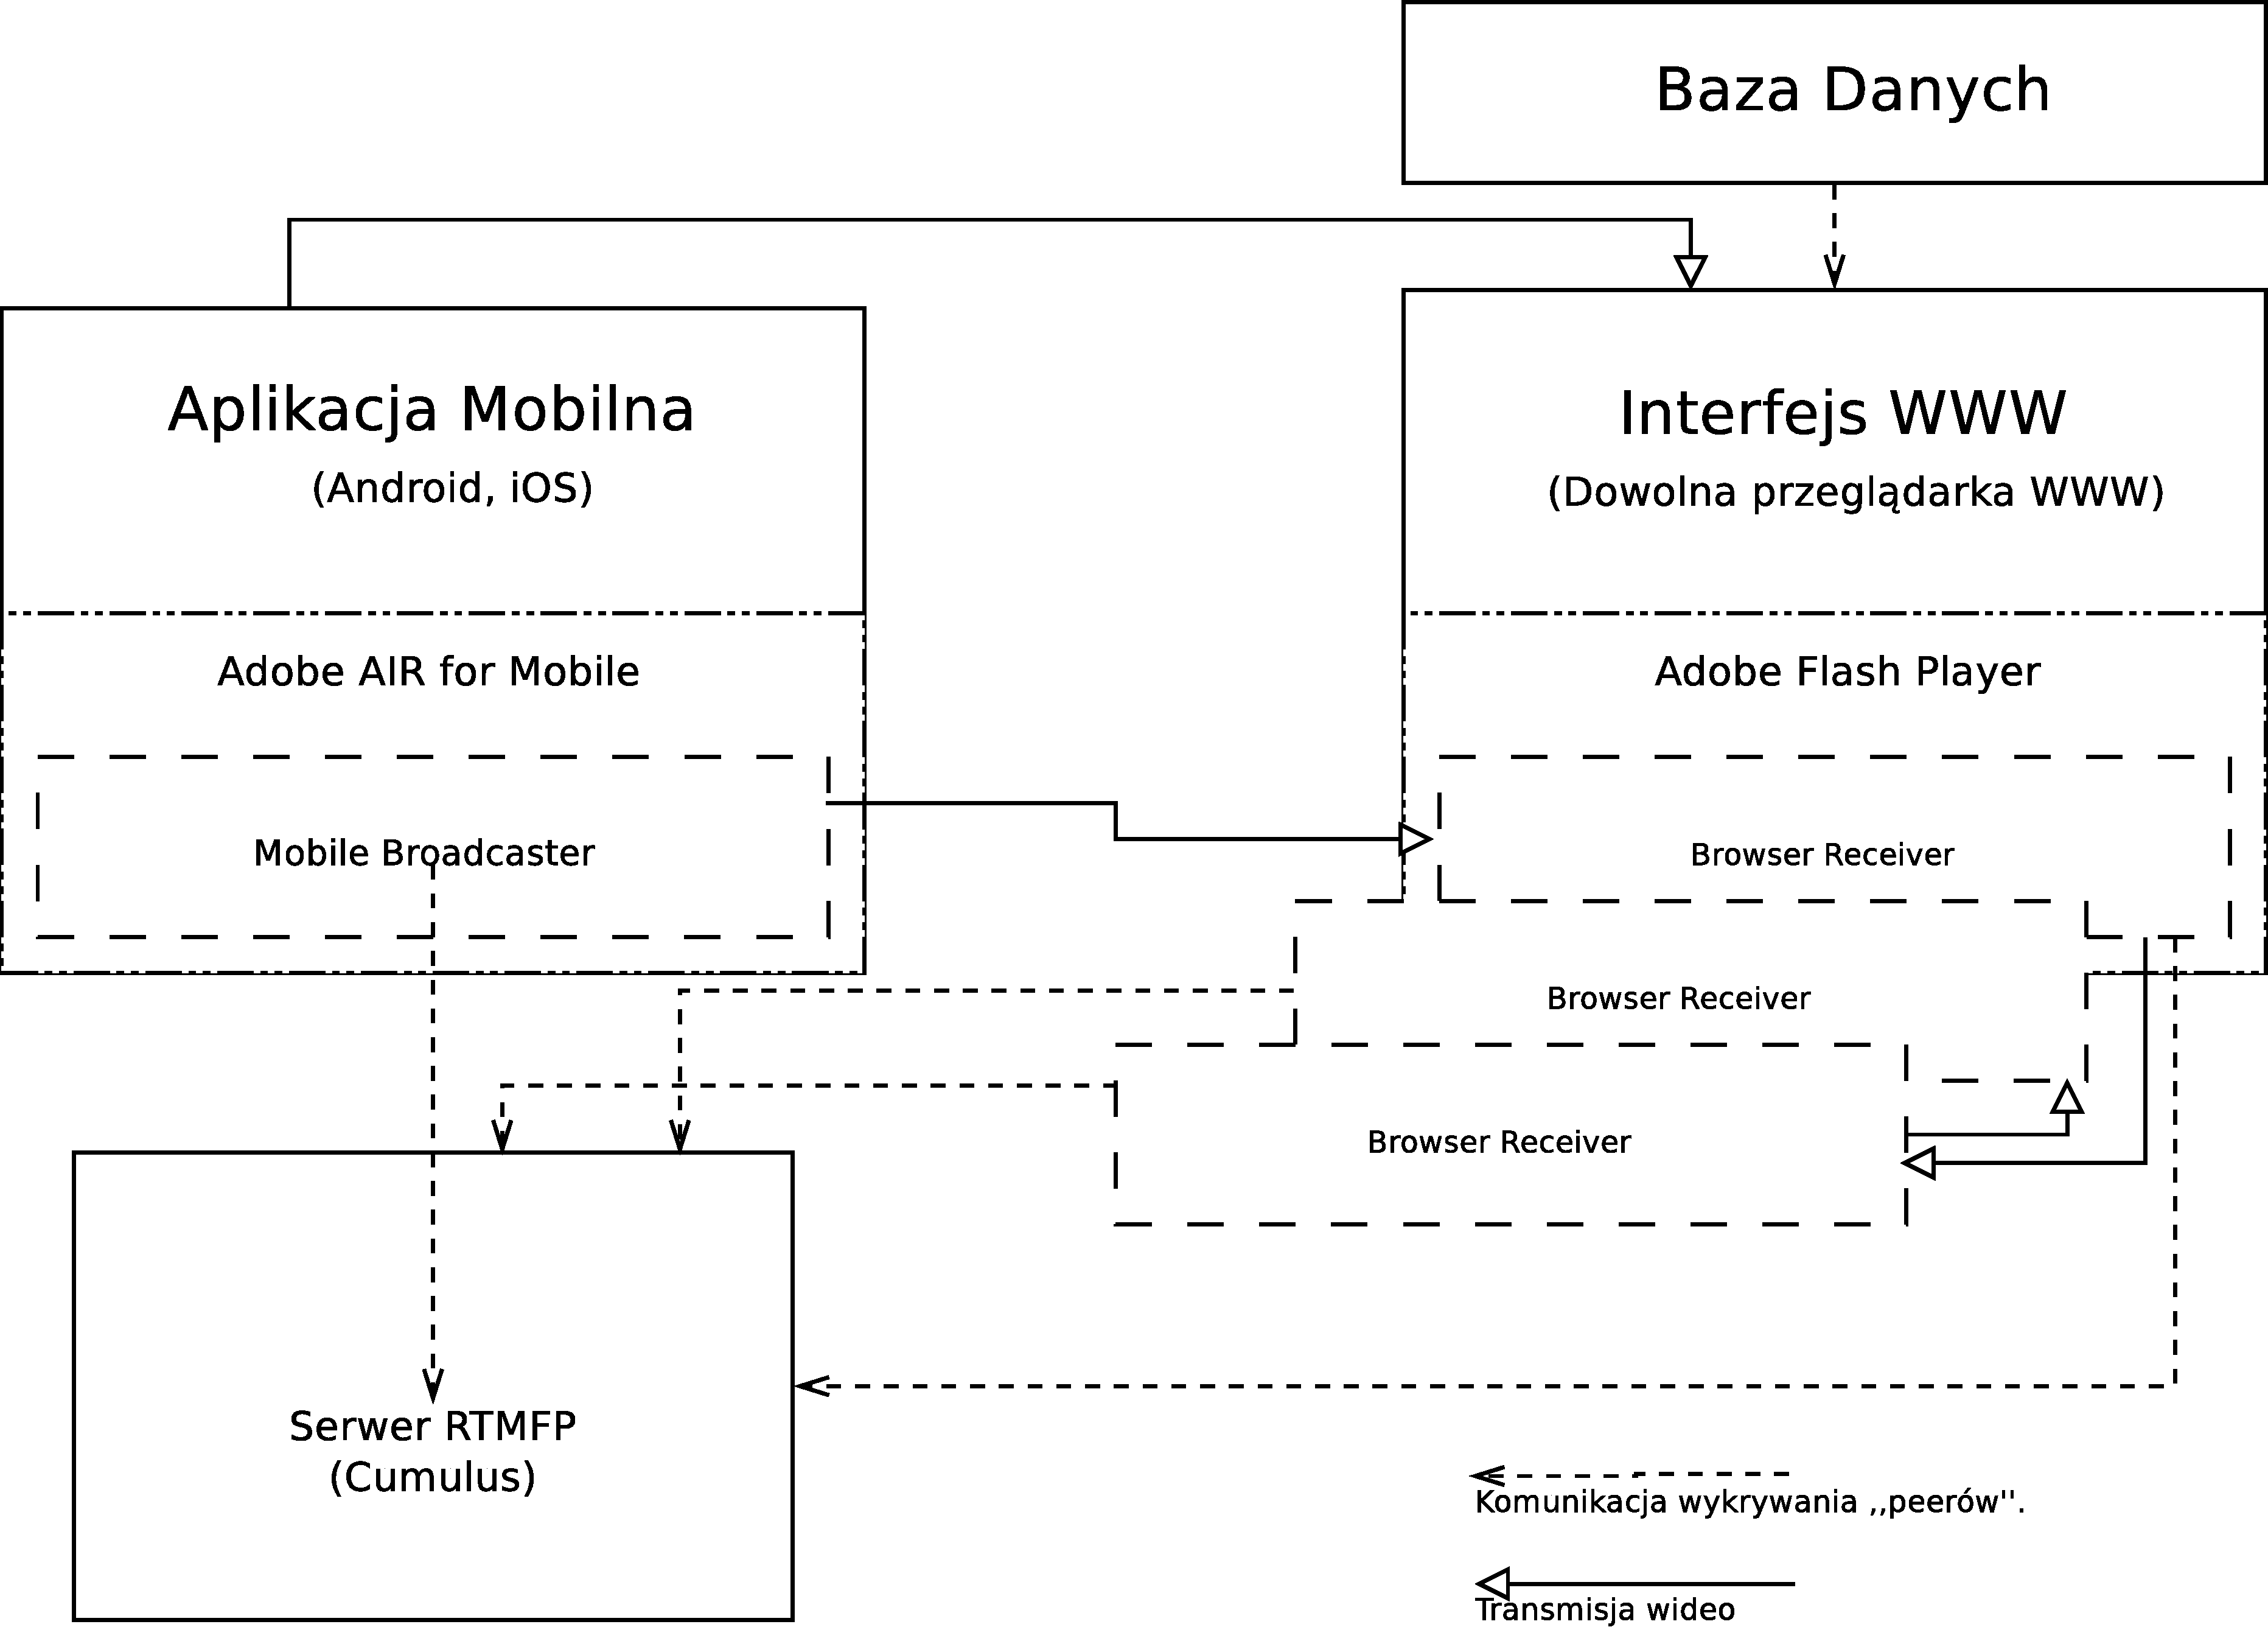
\includegraphics[width=\textwidth]{diagramy/architektura-implementacja.pdf}
    \captionof{figure}{Architektura implementacji prototypu systemu uwzględniająca transmisję wideo z Mobile Broadcastera do kilku Browser Receiverów.}
    \label{fig:architekturaImplementacji}
\end{center}

\subsection{Interfejs WWW}
Niżej przedstawiono elementy, które udało się zaimplementować w części systemu nazwanej Interfejs WWW. Szczegóły i opis architektury znajdują się \namedref{sec:EtapIwstepnaArchitekturaSystemu}.

\begin{packed_item}
    \item{System rejestracji użytkownika (\url{http://facewithme.com/accounts/register}), można zobaczyć na rysunku \ref{fig:rejestracja}.}
    \item{System logowania użytkownika (\url{http://facewithme.com/accounts/login}), można zobaczyć na rysunku \ref{fig:logowanie}.}
    \item{Panel administracyjny do zarządzania streamami, kategoriami i użytkownikami (\url{http://facewithme.com/admin}), można zobaczyć na rysunku \ref{fig:panelAdministracyjny}.}
    \item{Interaktywną mapę prezentującą streamy (\url{http://facewithme.com}), można zobaczyć na rysunku \ref{fig:interaktywnaMapa}.}
    \item{Funkcję automatycznej lokalizacji użytkownika i ustawienie pozycji mapy zgodnie z nią (\url{http://facewithme.com}), można zobaczyć na rysunku \ref{fig:interaktywnaMapa}.}
    \item{Listowanie wszystkich streamów nadawanych w systemie z podziałem na kategorie (\url{http://facewithme.com/stream/list}), można zobaczyć na rysunku \ref{fig:listaStreamow}.}
    \item{Wyświetlanie Browser Receivera, można zobaczyć na rysunku \ref{fig:browserReceiver}.}
\end{packed_item}

\begin{center}
    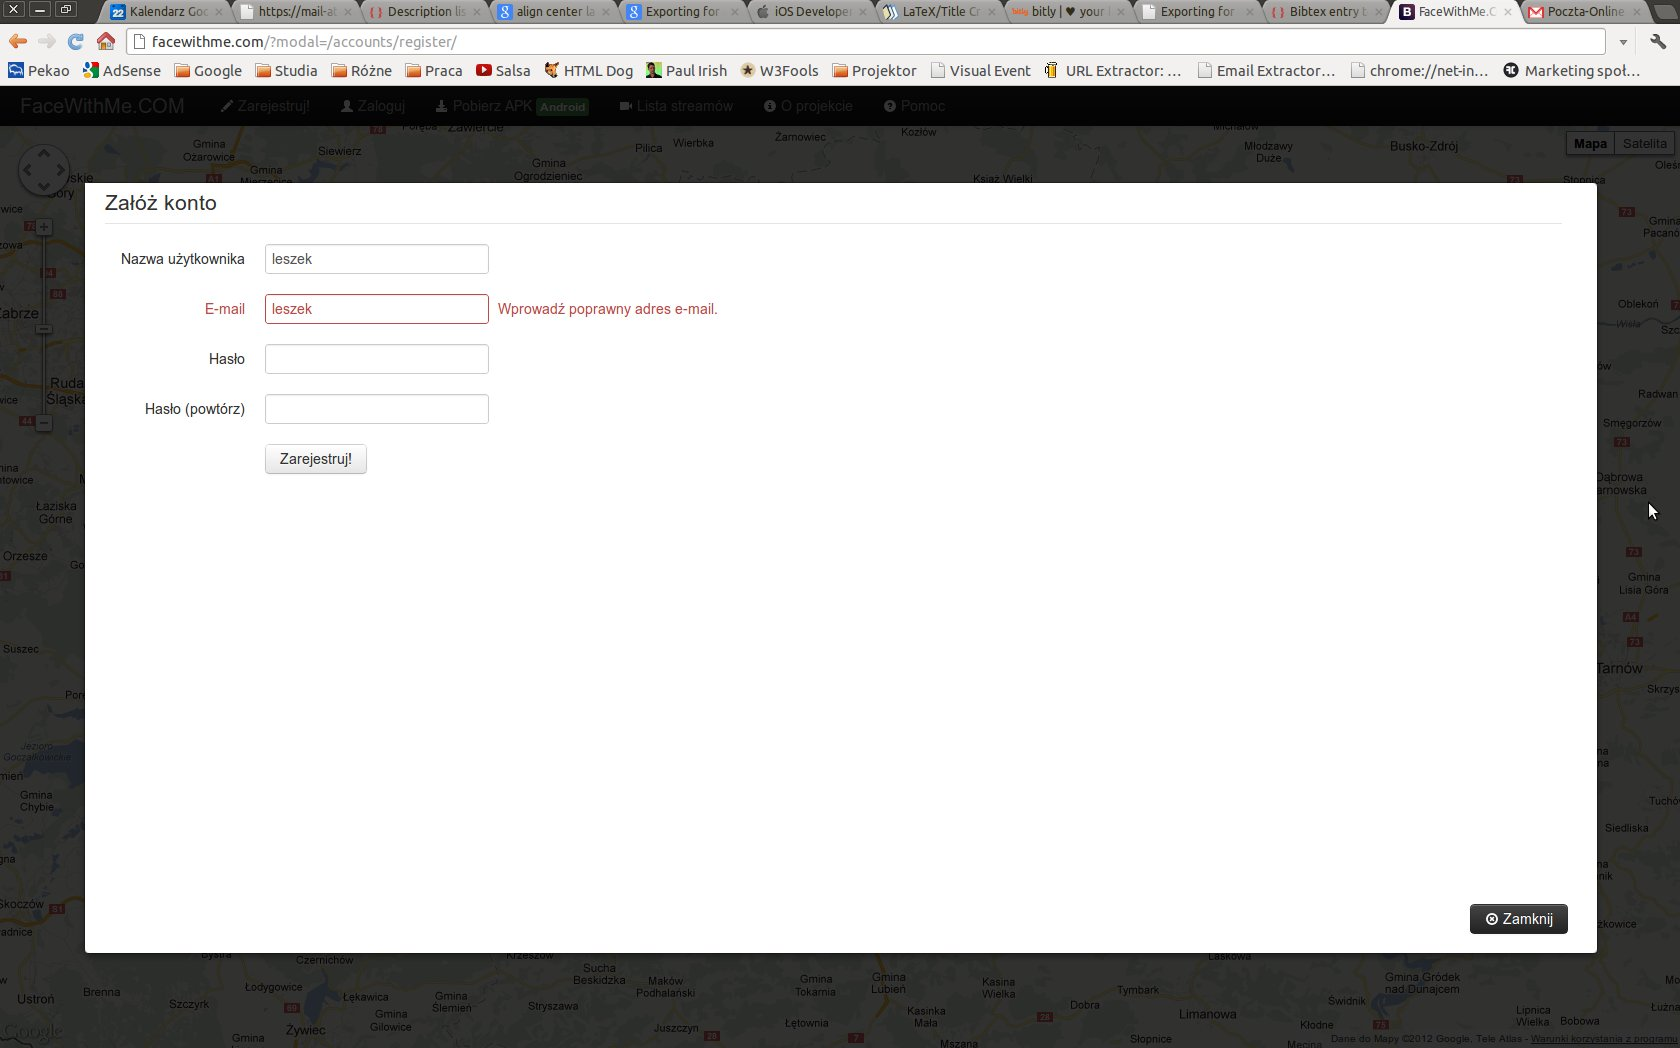
\includegraphics[width=\textwidth]{img/screens/interfejs_www/rejestracja.jpg}
    \captionof{figure}{System rejestracji użytkownika.}
    \label{fig:rejestracja}
\end{center}
\begin{center}
    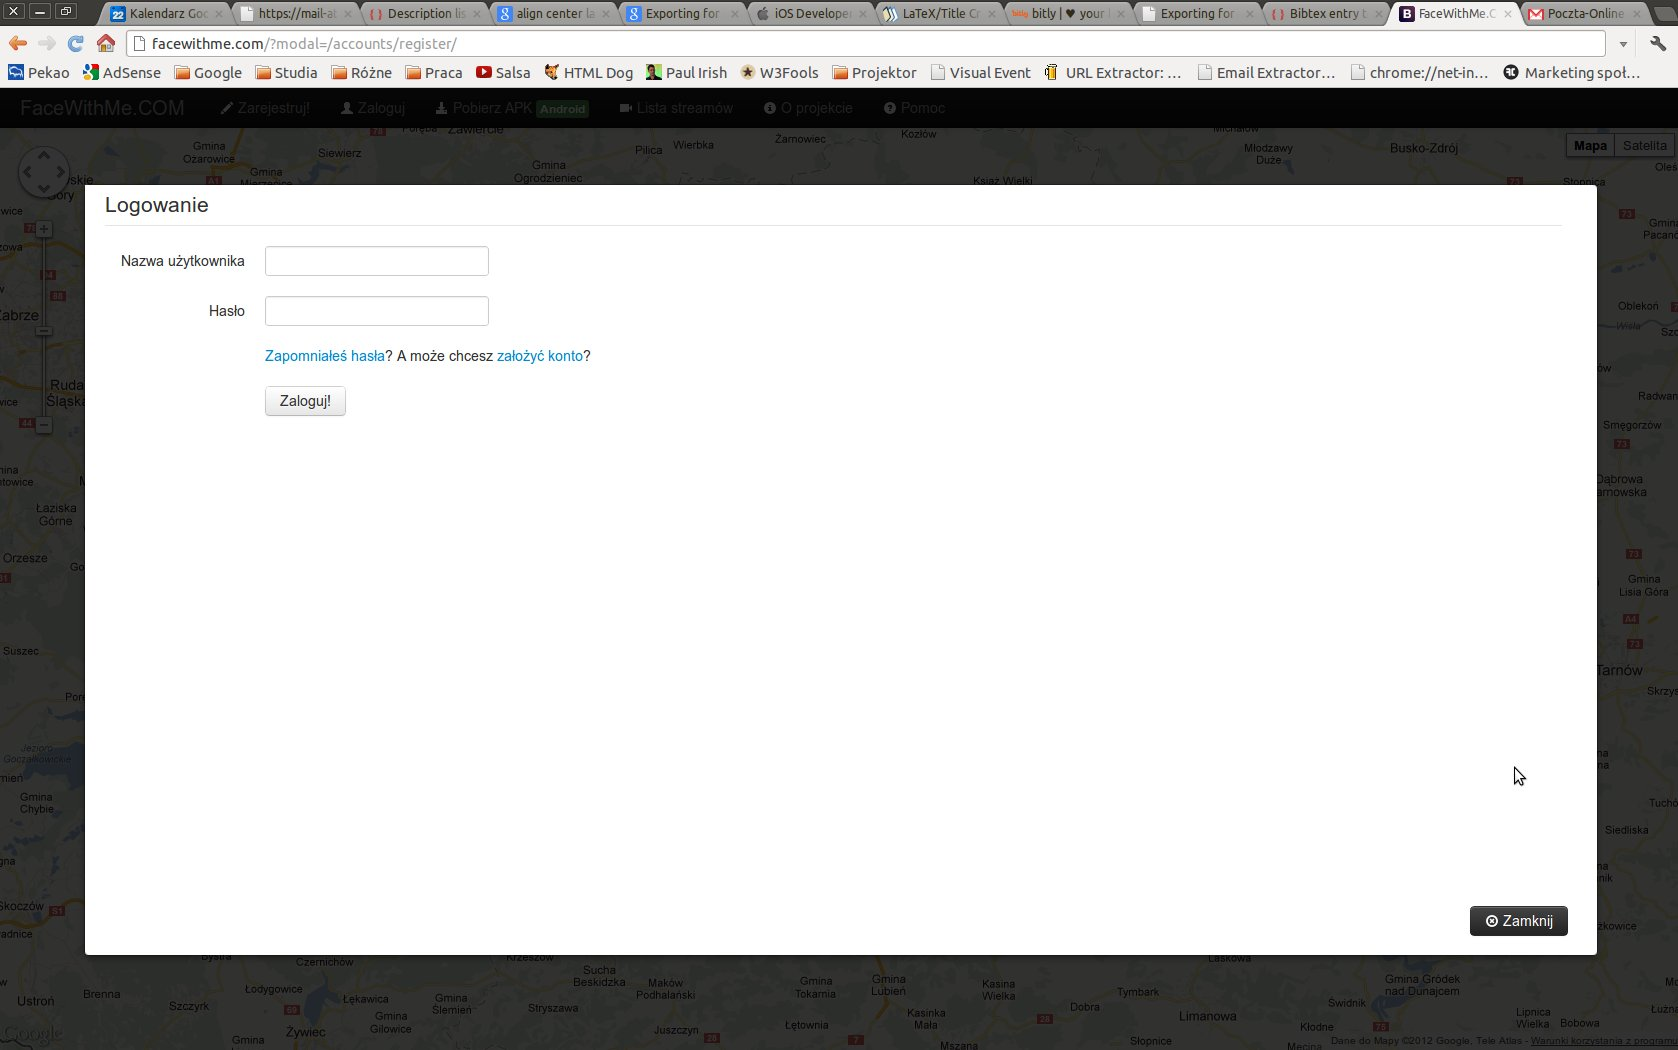
\includegraphics[width=\textwidth]{img/screens/interfejs_www/logowanie.jpg}
    \captionof{figure}{System logowania użytkownika.}
    \label{fig:logowanie}
\end{center}
\begin{center}
    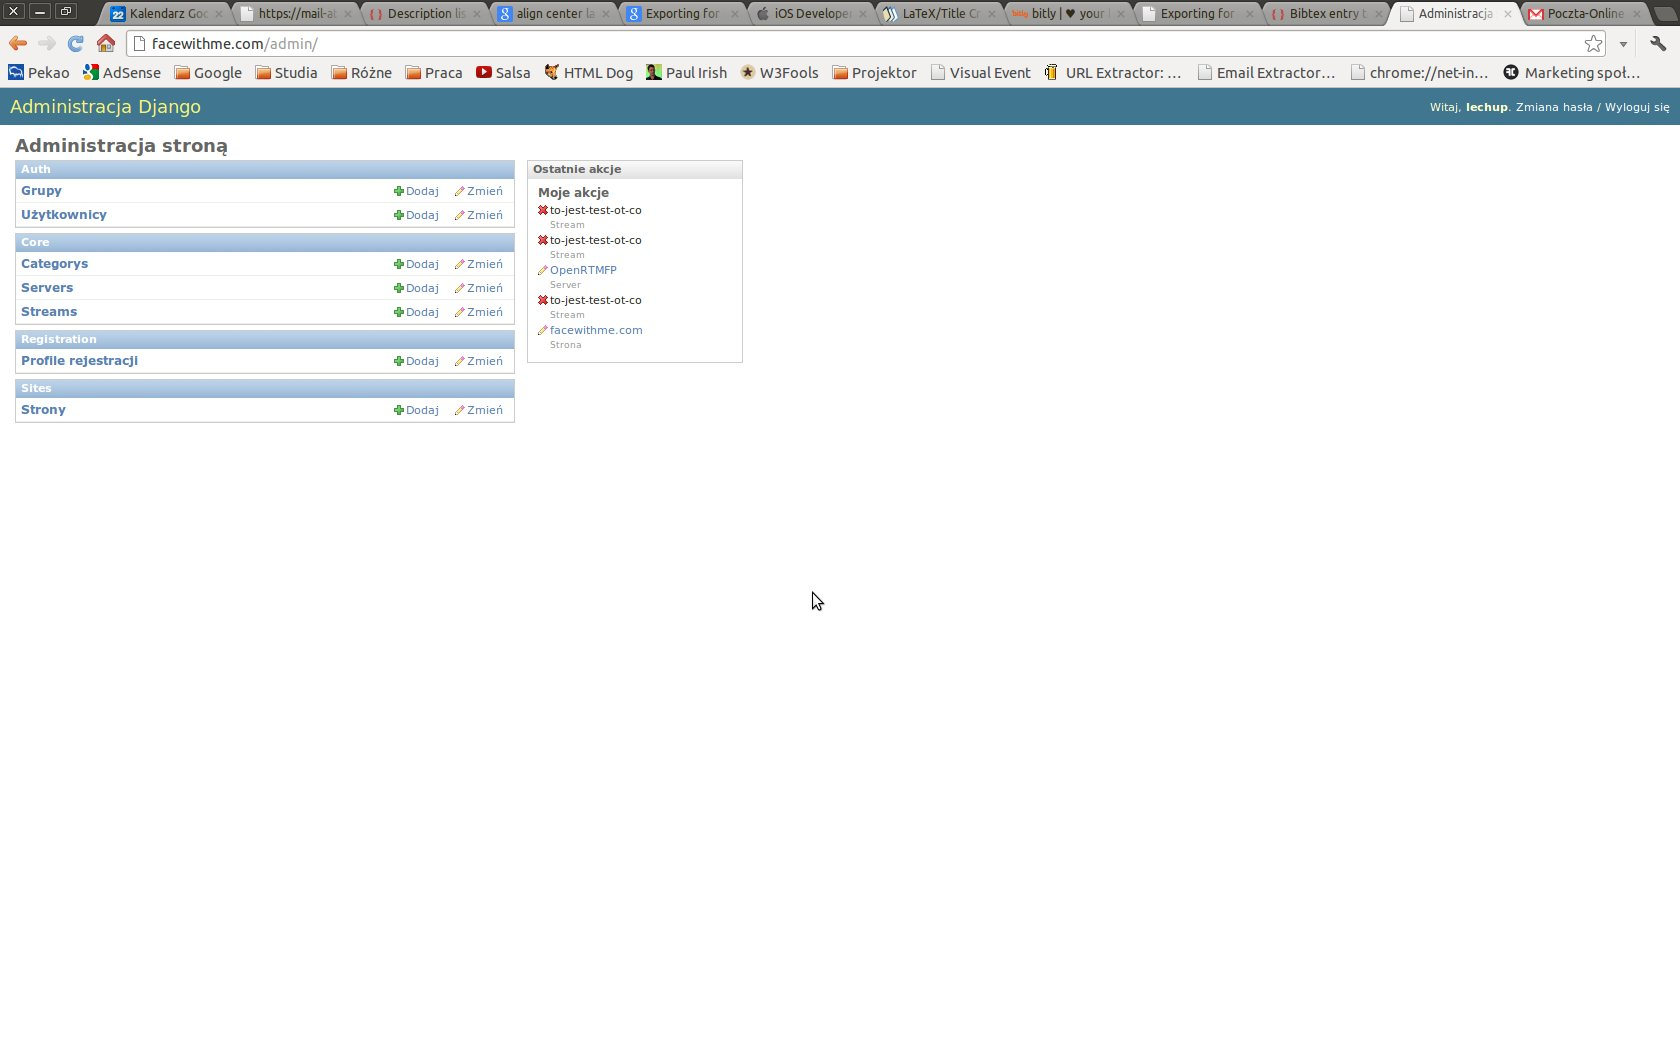
\includegraphics[width=\textwidth]{img/screens/interfejs_www/panel-administracyjny.jpg}
    \captionof{figure}{Panel administracyjny do zarządzania streamami, kategoriami i użytkownikami.}
    \label{fig:panelAdministracyjny}
\end{center}
\begin{center}
    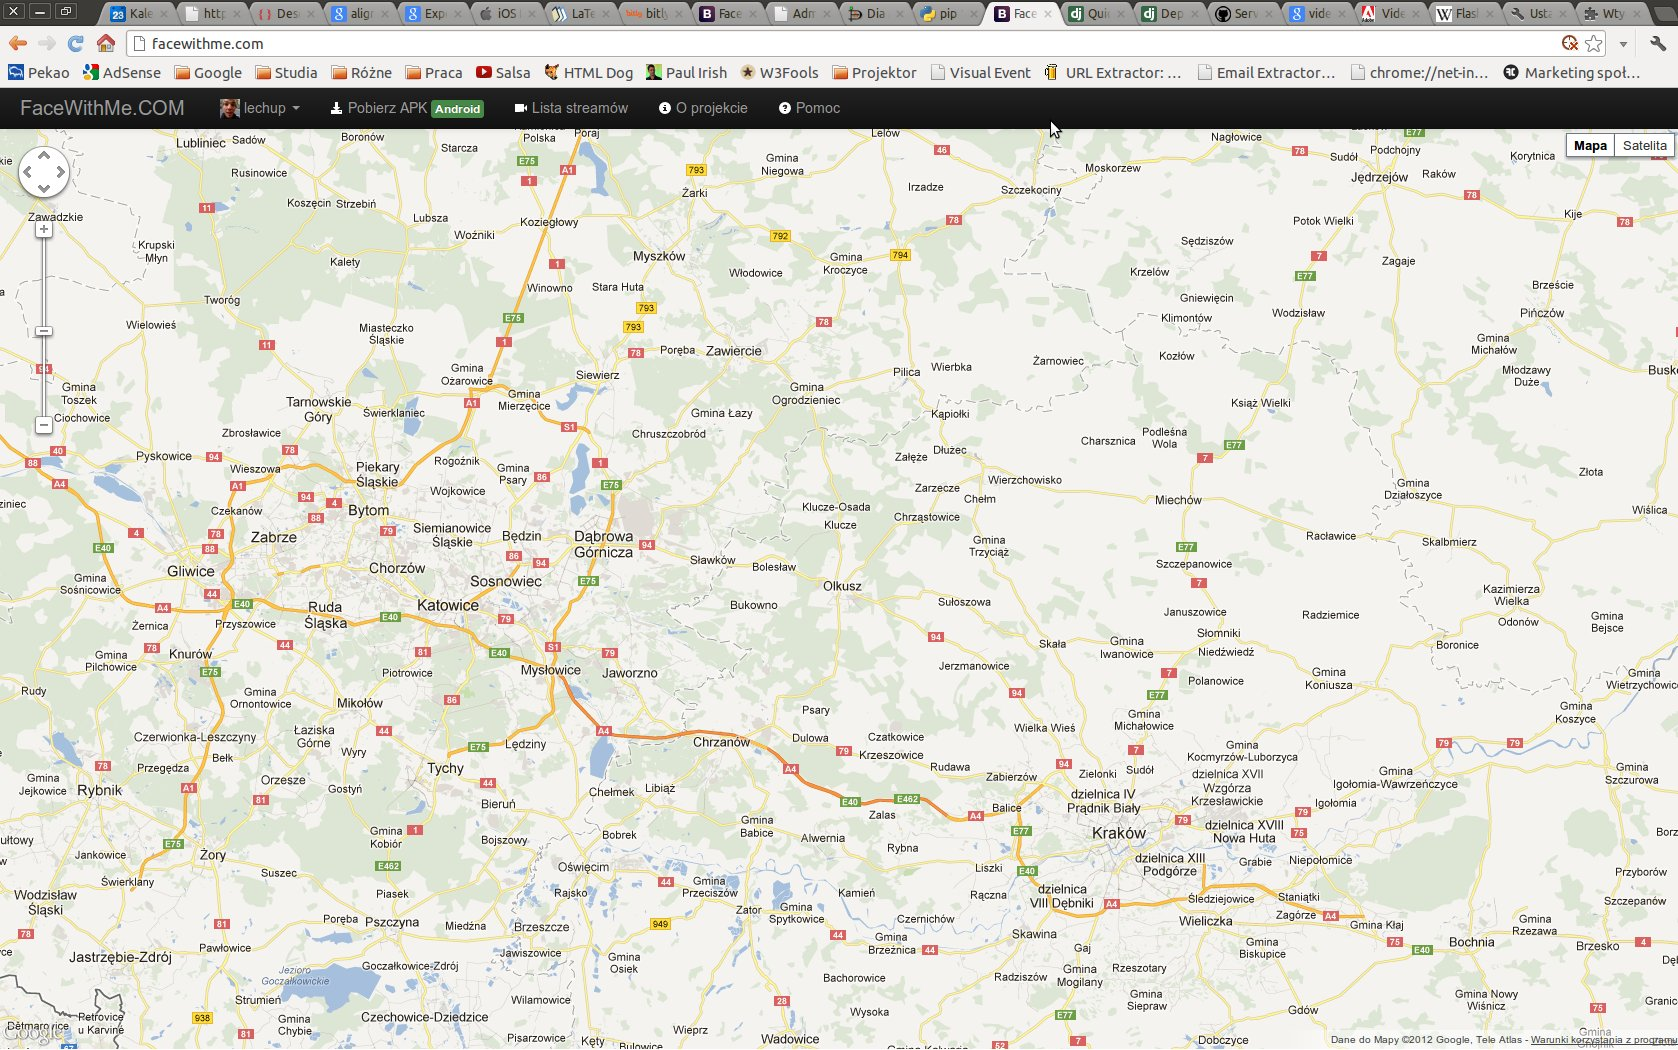
\includegraphics[width=\textwidth]{img/screens/interfejs_www/interaktywna-mapa.jpg}
    \captionof{figure}{Interaktywna mapa prezentująca streamy.}
    \label{fig:interaktywnaMapa}
\end{center}
\begin{center}
    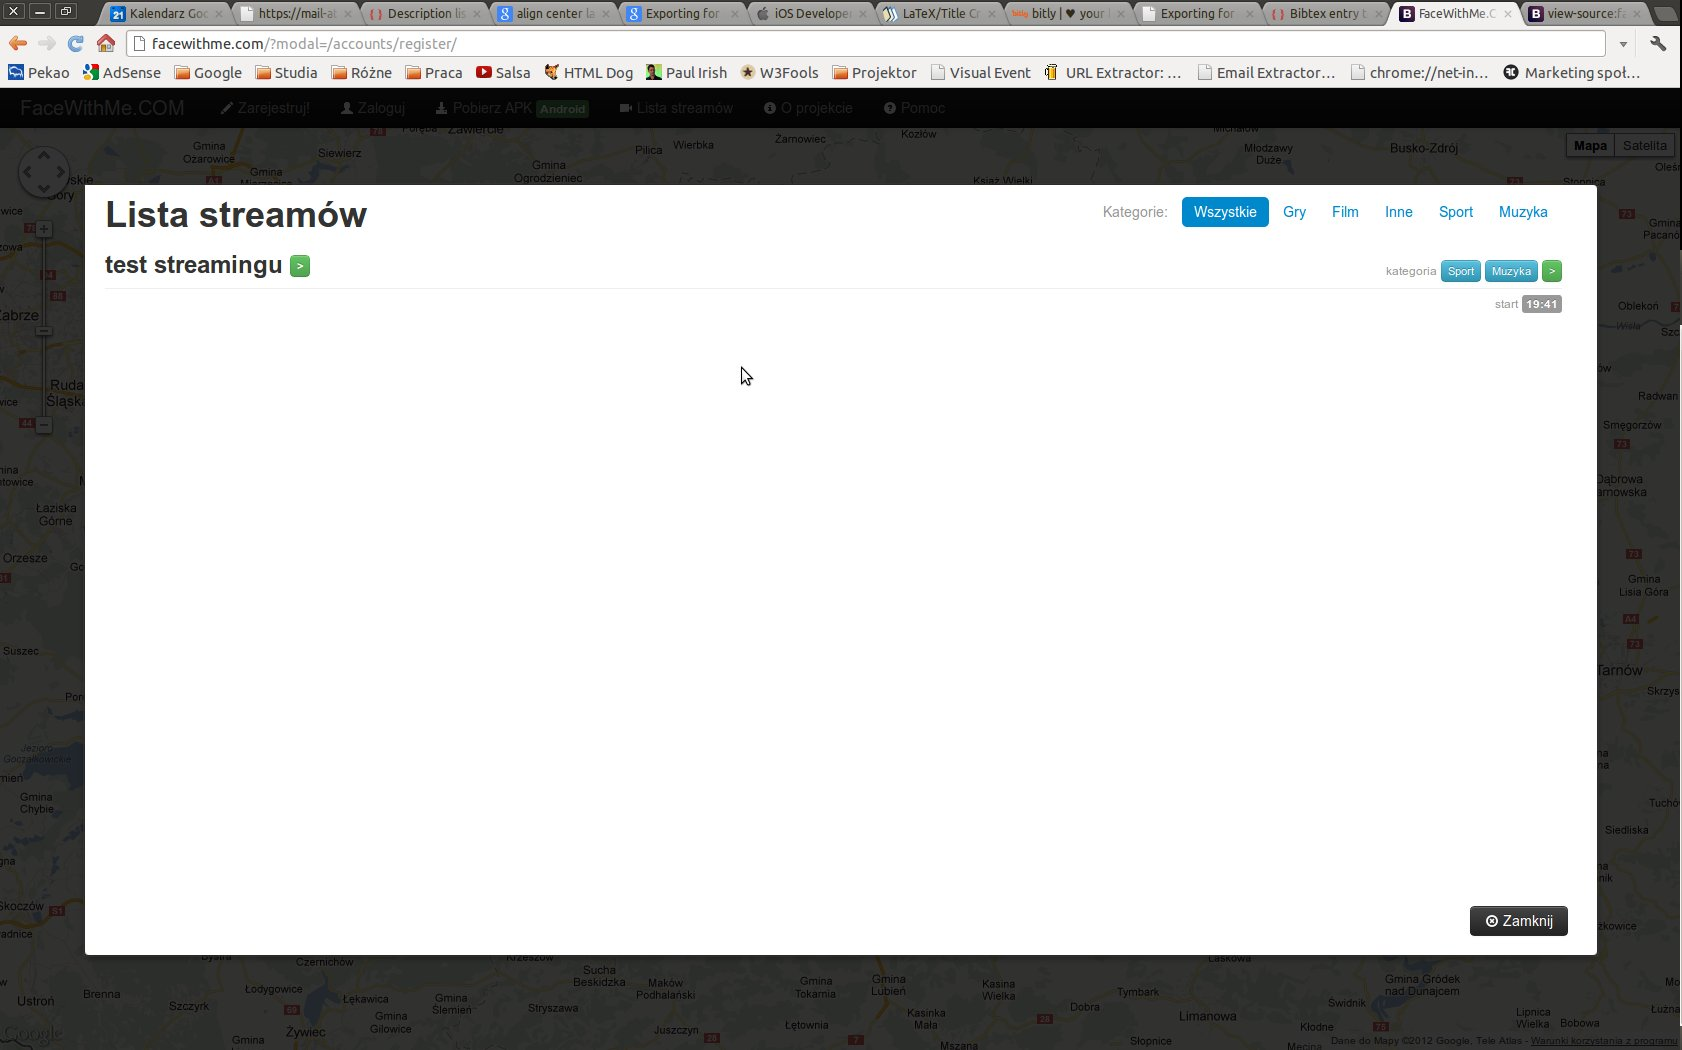
\includegraphics[width=\textwidth]{img/screens/interfejs_www/lista-streamow.jpg}
    \captionof{figure}{Lista streamów nadawanych w systemie z podziałem na kategorie.}
    \label{fig:listaStreamow}
\end{center}
\begin{center}
    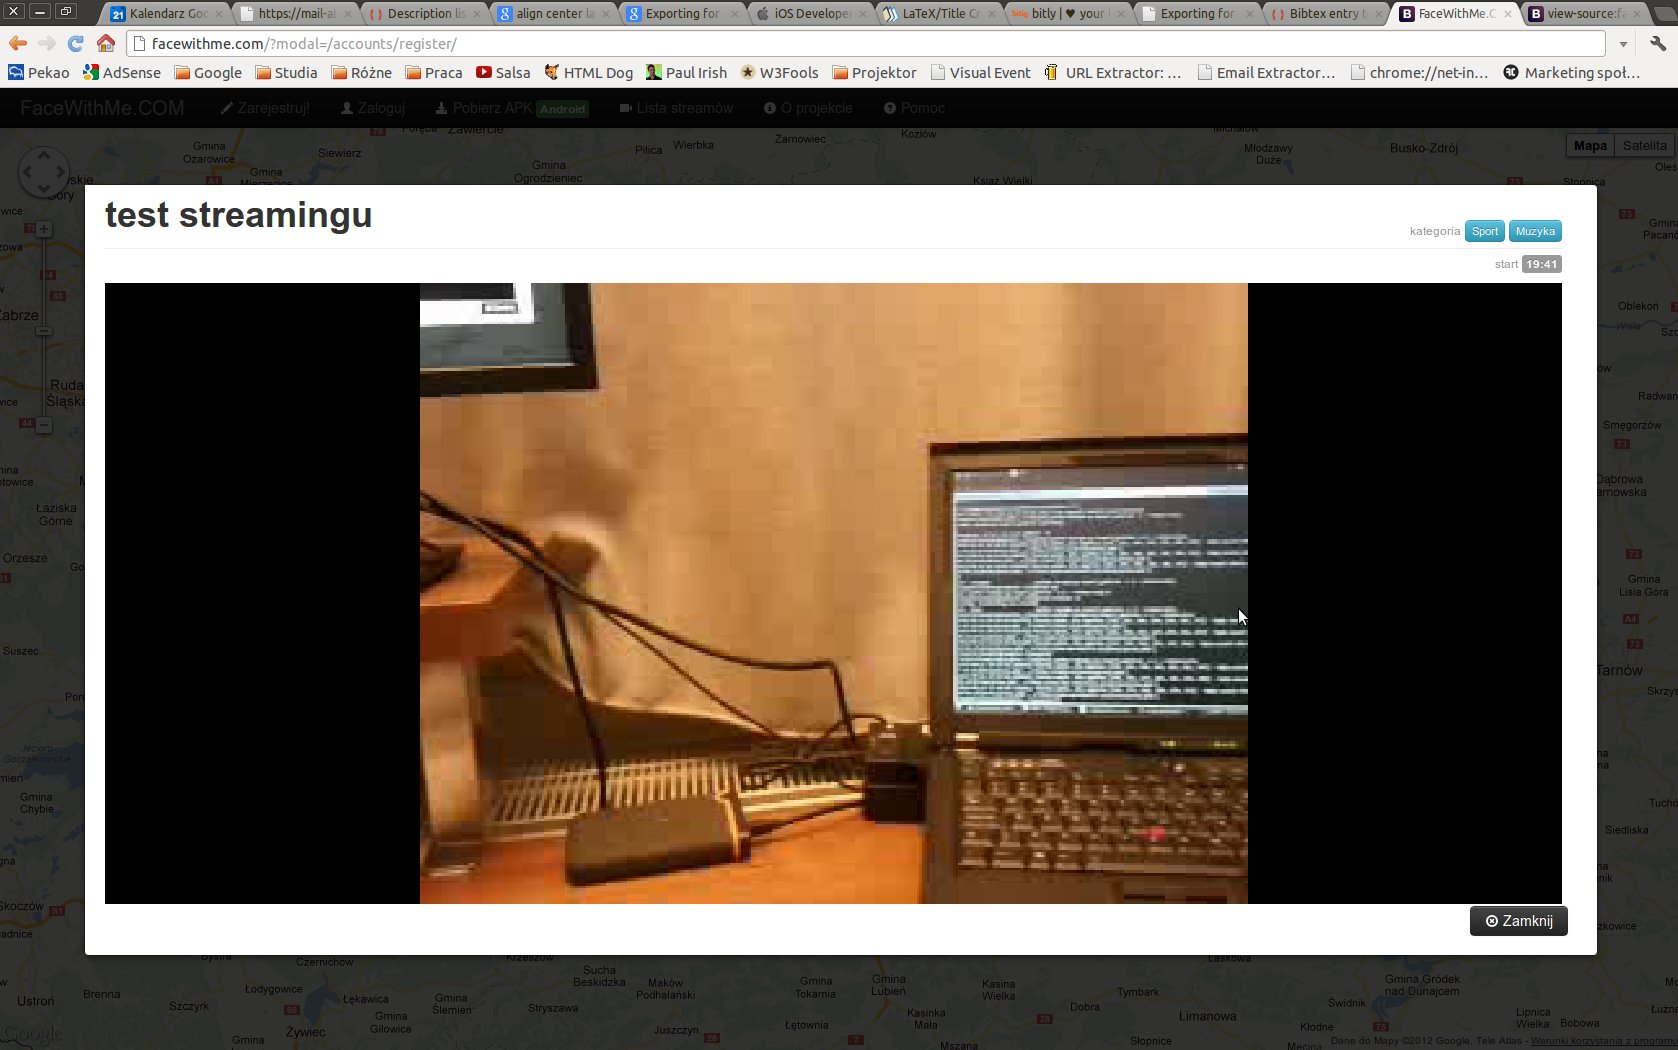
\includegraphics[width=\textwidth]{img/screens/interfejs_www/browser-receiver.jpg}
    \captionof{figure}{Wyświetlanie Browser Receivera w Google Chrome.}
    \label{fig:browserReceiver}
\end{center}


\newpage
\subsection{Mobile Broadcaster}
Mobile Broadcaster, czyli aplikacja umożliwiająca nadawanie streamu -- szczegóły \namedref{sec:EtapIwstepnaArchitekturaSystemu} -- jest aplikacją na systemy Android wykonana w środowisku AIR. Na przygotowanej stronie \url{http://facewithme.com} można pobrać aplikację. Aplikacji nie umieszczono w Google Play, gdyż nie jest ona produktem skończonym, a tylko takie można umieszczać na tej platformie. Aplikacja w formie instalatora na systemy Android została umieszczona również na dołączonej płycie CD w katalogu \texttt{./src/Django/facewithme/apps/core/static/FaceWithMe.apk}. Aplikacja została przetestowana z wykorzystaniem środowisk uściślonych w \namedref{sec:EtapIprzeprowadzoneTesty}. Niżej przedstawiono funkcje Mobile Broadcastera, które udało się zaimplementować w prototypie systemu.

\begin{packed_item}
    \item{Panel udostępniania streamu wideo, można zobaczyć na rysunku~\ref{fig:MB1}.}
    \item{Streaming wideo, można zobaczyć na rysunku~\ref{fig:MB2}.}
    \item{Ustawianie jakości streamu w trakcie nadawania, można zobaczyć na rysunku~\ref{fig:MB3}.}
    \item{Panel ustawień aplikacji, można zobaczyć na rysunku~\ref{fig:MB4}.}
    \item{Panel DEBUG aplikacji, można zobaczyć na rysunku~\ref{fig:MB5}.}
\end{packed_item}

\begin{figure}[h]
    \centering
    \begin{subfigure}{0.4\textwidth}
        \centering
        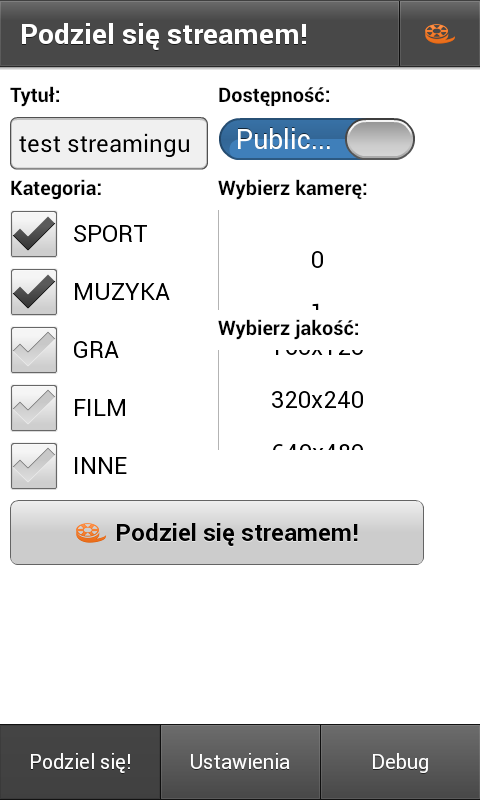
\includegraphics[width=\textwidth]{img/screens/mobile_broadcaster/panel-udostepniania-streamu.png}
        \caption{Panel udostępniania streamu.}
        \label{fig:MB1}
    \end{subfigure}
    \quad
    \begin{subfigure}{0.4\textwidth}
        \centering
        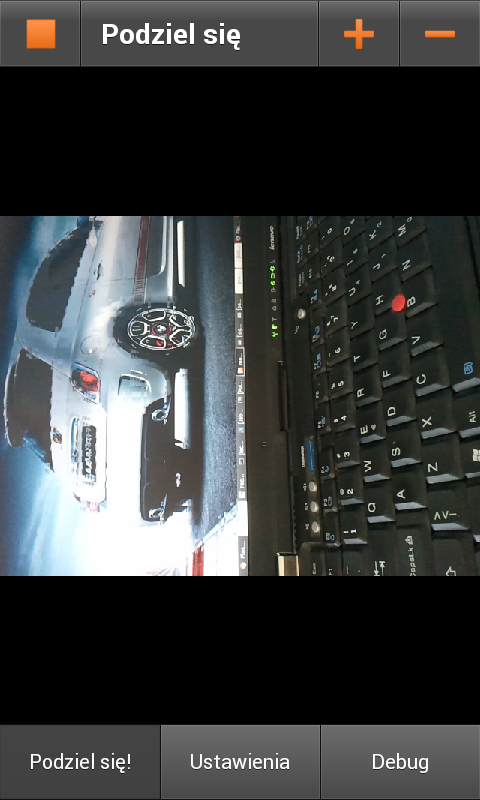
\includegraphics[width=\textwidth]{img/screens/mobile_broadcaster/streaming-wideo.png}
        \caption{Streaming wideo.}
        \label{fig:MB2}
    \end{subfigure}
    \caption{Screenshoty z Mobile Receivera część 1.}
\end{figure}

\begin{figure}[ht]
    \centering
    \begin{subfigure}{0.3\textwidth}
        \centering
        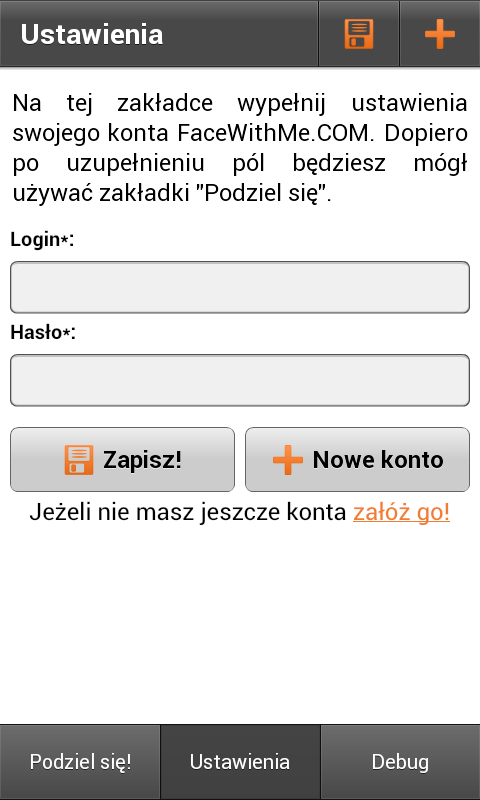
\includegraphics[width=\textwidth]{img/screens/mobile_broadcaster/panel-ustawien.png}
        \caption{Panel ustawień aplikacji.}
        \label{fig:MB3}
    \end{subfigure}
    \quad
    \begin{subfigure}{0.3\textwidth}
        \centering
        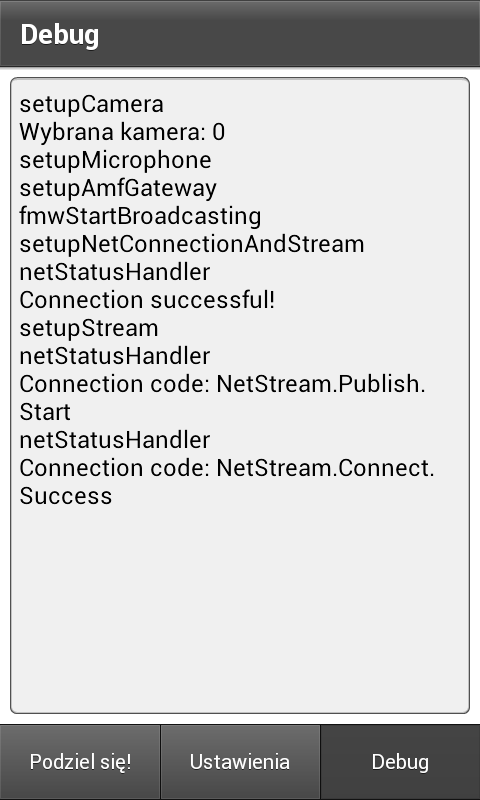
\includegraphics[width=\textwidth]{img/screens/mobile_broadcaster/panel-debug.png}
        \caption{Panel DEBUG aplikacji.}
        \label{fig:MB4}
    \end{subfigure}
    \quad
    \begin{subfigure}{0.3\textwidth}
        \centering
        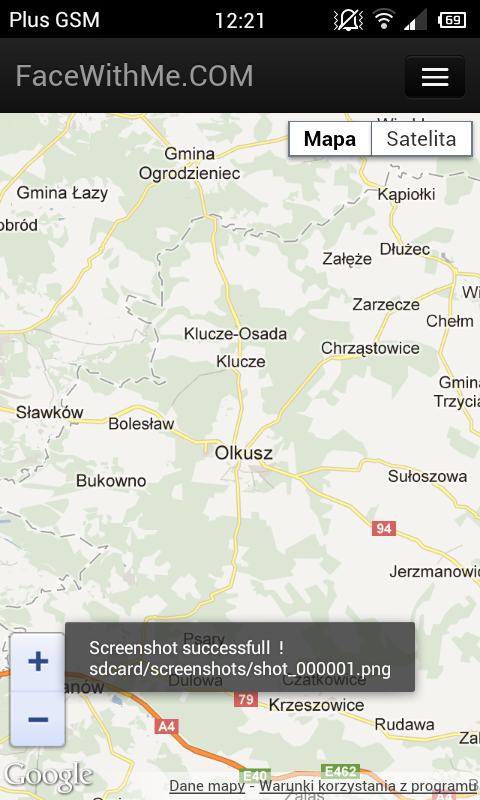
\includegraphics[width=\textwidth]{img/screens/mobile_broadcaster/interfejs-www.png}
        \caption{Interfejs WWW widoczny z poziomu przeglądarki mobilnej.}
        \label{fig:MB5}
    \end{subfigure}
    \caption{Screenshoty z Mobile Receivera część 2.}
\end{figure}

\newpage
\section{Co wymaga usprawnienia}
\label{sec:ImplementacjaPrototypuCoWymagaUsprawnienia}
Przy implementacji prototypu systemu, nie skupiano się na sprawach pobocznych jak interfejs czy komunikacja z użytkownikiem. Głównie kierowano się intencją przetestowania w praktyce działania technologii Adobe P2P Multicasting. Dlatego też system wymaga znacznej ilości poprawek zanim może zacząć być wykorzystywany publicznie. Przygotowany prototyp traktować można jako bazę wyjściową do zapoznania się z działaniem i wydajnością technologii. Główne braki prototypu systemu to:

\begin{packed_item}
    \item{Brak szyfrowania połączeń HTTP pomiędzy użytkownikiem a systemem, dotyczy także logowania.}
    \item{Brak jakiejkolwiek autoryzacji serwera RTMFP, jest dostępny publicznie.}
    \item{Brak zabezpieczenia publicznego/prywatnego streamu wideo.}
    \item{Brak całego Mobile Receivera, szczegóły \namedref{sec:EtapIwstepnaArchitekturaSystemu}.}
    \item{Brak całego Browser Broadcastera, szczegóły \namedref{sec:EtapIwstepnaArchitekturaSystemu}.}
    \item{Isnienie panelu DEBUG w Mobile Broadcasterze.}
    \item{Brak obrotu komponentu kamery względem obrócenia urządzenia w Mobile Broadcasterze co skutkuje przesuwaniem obrazu kamery góra/dół, gdy kamera fizycznie poruszana jest prawo/lewo.}
    \item{Brak automatycznego usuwania streamu z Interfejsu WWW w przypadku nieoczekiwanego przerwania działania Mobile Broadcastera.}
    \item{Brak komunikatów skierowanych do użytkownika Mobile Broadcastera, informujących o stanie lub błędach aplikacji.}
    \item{Brak wyłączania trybu czuwania urządzenia podczas udostępniania streamu.}
    \item{Brak aplikacji na iOS -- Głównym powodem dla którego nie udało się stworzyć i przetestować aplikacji na platformę iOS jest koszt licencji Apple Developer Account (99\$), jaki trzeba ponieść, aby dostać możliwość umieszczania aplikacji na Apps Market oraz testowania aplikacji na własnym telefonie (szczegóły można znaleźć \cite{UnknAuth11}). Z powodu zastosowania technologii Adobe AIR for Mobile, nie ma możliwości testowania aplikacji za pomocą XCode i wirtualnego środowiska iOS. Z tego powodu dostępność komputerów Mac na uczelni na wiele się nie zdała.}
    \item{Brak środowiska testującego oraz testów kodu źródłowego Adobe Flash Platform, zarówno kodu Adobe AIR for Mobile jak i Adobe Flash.}
\end{packed_item}

\newpage
\section{Dokumentacja}
Zgodnie z filozofią metodyki \textit{XP} (szczegóły \namedref{sec:ZMTOzalozenia}), dokumentacja projektu sprowadza się do opisu architektury oraz komentarzy kodu, testów oraz komentarzy do testów. Unika się tworzenia bazy wiedzy, która najczęściej jest po pewnym czasie nieaktualizowana.

Dlatego też, aby zapoznać się z działaniem systemu należy przejrzeć architekturę systemu, a następnie zapoznać się bezpośrednio z kodem źródłowym i zawartymi w nim komentarzami.

\subsection{Uruchomienie systemu}

Aby uruchomić system z kodu źródłowego należy przygotować szereg aplikacji i skonfigurować odpowiednio środowisko. Niżej prezentowana jest lista części systemu, wraz z opisem jak daną część uruchomić.

\begin{description}
    \item[Interfejs WWW] Uruchomić aplikację Django, znajdującą się w dołączonym kodzie źródłowym w katalogu \texttt{./src/Django/facewithme/}. Wymagane do uruchomienia biblioteki środowiska Pythonowskiego w formacie pliku wymagań programu PIP znajdują się w \texttt{./src/Django/facewithme/requirements/requirements.txt}. Instrukcja instalacji i wdrożenia aplikacji Django znajduje się w \cite{DjangoDocs}. System wdrożony został przy wykorzystaniu Django 1.4.1.
    \item[Baza danych] Uruchomić i zainstalować serwer PostgreSQL (\cite{PostgreSQL}). Zainstalować rozszerzenie GIS zgodnie z instrukcją zamieszczoną w \cite{DjangoPostGIS}. System wdrożony został przy wykorzystaniu PostgreSQL 9.1.
    \item[Serwer RTMFP] Uruchomić serwer Cumulus. Instrukcja instalacji znajduje się w \cite{CumulusInstall}. Dodatkowo należy umieścić serwer na liście dostępnych serwerów w panelu administracyjnym aplikacji Django. Domyślnie, dodawane streamy losują jeden z dostępnych serwerów RTMFP. Można pokusić się o implementację algorytmu rozkładającego obciążenie bardziej równomiernie np. Round Robin.
    \item[Browser Receiver] Należy tak skonfigurować dołączanie obiektu flash, aby przekazywać informację na temat AMFGateway. Można do tego wykorzystać zmienną amfgateway dodając ją w widokach wyświetlających Browser Receiver. Domyślnie ustawiona jest na wartość \texttt{http://facewithme.com/amf/}.
    \item[Mobile Broadcaster] Należy uruchomić, zainstalować i skonfigurować środowisko Flash Develop zgodnie z tą instrukcją \cite{flashDevelopConfig}. W plikach źródłowych odnaleźć domyślną konfigurację AMFGateway (\texttt{./src/Flex/FaceWithMe Mobile/src/Main.mxml}) i poprawić ją na adres skonfigurowanego wcześniej Interfejsu WWW. Skompilować projekt oraz stworzyć odpowiednie paczki instalacyjne dla platform docelowych (Android / iOS).
\end{description}

W razie problemów z wyświetlaniem się streamu należy zapoznać się z plikiem pomocy \url{http://facewithme.com/help/}.

\subsection{Testy automatyczne}

Część Interfejsu WWW systemu posiada zalążki testów jednostkowych. Dotyczą one poprawnego wyświetlania widoków. Aby uruchomić testy, należy przejść do katalogu z z kodem źródłowym Django (\texttt{./src/Dajango/facewithme/}), a następnie uruchomić polecenie:

\lstset{language=Bash}
\begin{lstlisting}
python manage.py test core
\end{lstlisting}

O poprawnym wykonaniu testów informuje nas konsola, której wyjście zawiera:
\begin{lstlisting}
Creating test database for alias 'default'...
......
----------------------------------------------------------------------
Ran 6 tests in 0.822s

OK
Destroying test database for alias 'default'...
\end{lstlisting}

\subsection{Przeprowadzone testy}
\label{sec:EtapIprzeprowadzoneTesty}
System testowany był na kilku platformach. Niżej znajduje się lista konfiguracji systemu, w której poszczególne części nie wykazywały błędnego zachowania.

\begin{description}
    \item[Interfejs WWW z Browser Receiver] Google Chrome (21.0.1180.89) + Flash Player (11.3.31.232)/Linux; FireFox 15.0.1 + Flash Player 11.2.202.238/Linux; Google Google Chrome (21.0.1180.89) + Flash Player (11.3.31.232)/Windows 7;  FireFox 15 + Flash Player 11.2.202.238/Windows 7.
    \item[Mobile Broadcaster] Adobe AIR 3.4.0.254/Android 4.04/Samsung Galaxy S I, Adobe AIR 3.4.0.254/Android 3.2/Samsung Galaxy Tab 10.1.
\end{description}

\subsection{Bezpieczeństwo}
\label{sec:ImplementacjaPrototypuBezpieczenstwo}
Bardzo ważnym aspektem docelowego systemu powinno być bezpieczeństwo. Niżej wyszczególniono elementy prototypu systemu, które mają bezpośredni związek z bezpieczeństwem i sugerowane poprawki, które pomogą zabezpieczyć system.

\begin{packed_item}
    \item{Dzięki zastosowaniu technologii Adobe Flash Platform oraz wykorzystaniu protokołu RTMFP, transmisja danych pomiędzy Mobile Broadcasterem oraz Browser Receiverem jest szyfrowana. Szyfrowanie odbywa się za pomocą 128-bitowego klucza. Szczegółowe informacje można uzyskać w \cite{AdobeSecurity}}.
    \item{Komunikacja pomiędzy Interfejsem WWW, a Browser Receiverem oraz Mobile Receiverem, odbywająca się za pomocą AMFGateway powinna odbywać się za pomocą protokołu HTTPS, nie HTTP jak w prototypie.}
    \item{Logowanie do panelu administracyjnego oraz logowanie użytkowników powinno wykorzystywać protokół HTTPS, nie HTTP jak w prototypie.}
    \item{Sugeruje się przejście na HTTPS w każdej komunikacji nawiązywanej pomiędzy użytkownikiem, a Interfejsem WWW, nie HTTP jak w prototypie.}
    \item{Serwer RTMFP (Cumulus), nie udostępnia żadnego sposobu na autoryzację połączeń. Najprostszym sposobem na ograniczenie wykorzystania przez nieautoryzowanych użytkowników jest sprawdzanie \texttt{swfUrl} połączającego się klienta za pomocą rozszerzenia serwera wykorzystującego zdarzenie \texttt{onConnection} (szczegóły w \cite{CumulusDocs}).}
\end{packed_item}

\newpage
\section{Wydajność P2P Multicasting w Adobe Flash Platform}
\label{sec:ImplementacjaPrototypuWydajnoscP2P}
W tym rozdziale chciano poruszyć temat związany z wydajnością transmisji wideo za pomocą technologii P2P Multicasting. Kryterium jakie chcemy sprawdzać to opóźnienie transmisji wideo względem obrazu oryginalnego oraz jego płynność. Opóźnienie jest wyrażone w sekundach. Płynność określono jako jedną z poniższych możliwości.
\begin{description}
    \item[Obraz całkowicie płynny] Obraz zachowuje płynność ciągle.
    \item[Obraz płynny] Obraz od czasu do czasu wstrzymuje się, większą część czasu jest płynny.
    \item[Obraz skaczący] Obraz nie jest płynny, posiada natomiast więcej niż jedną klatkę na sekundę.
    \item[Obraz poklatkowy] Obraz nie jest całkowicie płynny, posiada mniej niż jedną klatkę na sekundę.
    \item[Obraz nieczytelny] Obraz pojawia się we fragmentach, wyświetlają się pomniejsze.
\end{description}

Środowisko testowe składa się z dwóch komputerów klientów, na których uruchomiono przeglądarkę Google Chrome i włączono Browser Receiver dla streamu udostępnianego przez Mobile Broadcaster uruchomionego na Adobe AIR 3.4.0.254/Android 3.2/Samsung Galaxy Tab 10.1. Aplikacja mobilna wysyłanie streamu wideo przeprowadza za pomocą łącza ADSL (połączenie WiFi przez router) o parametrach faktycznych 8 Mb/s pobieranie, 1 Mb/s wysyłanie danych. Alternatywnym połączeniem Mobile Broadcastera jest darmowy internet od Aero2 w technologii HSPA/HSPA+ o parametrach faktycznych 0.5 Mb/s pobieranie, 0.4 Mb/s wysyłanie danych. Komputery klienckie są połączone do tej samej sieci LAN, korzystającej z wcześniej wymienionego łącza ADSL. Test prędkości łącz został wykonany za pomocą serwisu \url{http://speedtest.net}. W poniższej tabeli znajdują się parametry łącz na których przeprowadzono testy.

\begin{table}[h]
    \centering
    \begin{tabular}{|l|l|l|l|}
        \hline
        & ping & prędkość pobierania & prędkość wysyłania \\
        \hline
        ADSL
        &
        51~ms
        &
        8~Mb/s
        &
        1~Mb/s
        \\
        \hline
        Aero2
        &
        107~ms
        &
        0.5~Mb/s
        &
        0.4~Mb/s
        \\
        \hline
    \end{tabular}
    \caption{Parametry łącz na których zostały przeprowadzone testy.}
\end{table}

Wpływ na badane kryteria mają parametry:
\begin{packed_item}
    \item{Rozdzielczość obrazu w transmisji wideo, która jest przekazywana.}
    \item{Ilość klientów uczestniczących w transmisji P2P Multicast.}
    \item{Łącze wykorzystywane przez Mobile Broadcastera.}
    \item{Łącze wykorzystywane przez Browser Receivera.}
\end{packed_item}

Tabela przedstawiająca płynność transmisji oglądanej na ekranie Browser Receivera, względem rozdzielczości przesyłanego strumienia w pikselach. Dla dwóch włączonych Browser Reveiverów, po jednej instancji per komputer klient:
\begin{table}[h]
    \centering
    \begin{tabular}{|l|l|l|l|l|}
        \hline
        & 80x60px & 160x120px & 320x240px & 640x480px \\
        \hline
        ADSL
        &
        obraz całkowicie płynny 
        &
        obraz całkowicie płynny
        &
        obraz płynny
        &
        obraz skaczący
        \\
        \hline
        Aero2
        &
        obraz płynny
        &
        obraz poklatkowy
        &
        obraz nieczytelny
        &
        obraz nieczytelny
        \\
        \hline
    \end{tabular}
    \caption{Płynność transmisji wideo w danej rozdzielczości względem wykorzystywanego łącza dla dwóch Browser Receiverów.}
\end{table}

Tabela przedstawiająca opóźnienie transmisji oglądanej na ekranie Browser Receivera, względem rozdzielczości przesyłanego strumienia w pikselach. Dla dwóch włączonych Browser Reveiverów, po jednej instancji per komputer klient:
\begin{table}[h]
    \centering
    \begin{tabular}{|l|l|l|l|l|}
        \hline
        & 80x60px & 160x120px & 320x240px & 640x480px \\
        \hline
        ADSL
        &
        opóźnienie 0s
        &
        opóźnienie 0s
        &
        opóźnienie 0,1s
        &
        opóźnienie 0-1s \\
        \hline
        Aero2
        &
        opóźnienie 0,1-0,5s
        &
        opóźnienie 2-3s
        &
        opóźnienie 4-5s
        &
        opóźnienie ~40s \\
        \hline
    \end{tabular}
    \caption{Opóźnienie transmisji wideo w danej rozdzielczości względem wykorzystywanego łącza dla dwóch Browser Receiverów.}
\end{table}

Tabela przedstawiająca płynność transmisji oglądanej na ekranie Browser Receivera, względem rozdzielczości przesyłanego strumienia w pikselach. Dla sześciu włączonych Browser Reveiverów, po trzy instancje per komputer klient:
\begin{table}[h]
    \centering
    \begin{tabular}{|l|l|l|l|l|}
        \hline
        & 80x60px & 160x120px & 320x240px & 640x480px \\
        \hline
        ADSL
        &
        obraz całkowicie płynny 
        &
        obraz płynny
        &
        obraz płynny
        &
        obraz poklatkowy
        \\
        \hline
        Aero2
        &
        obraz płynny
        &
        obraz poklatkowy
        &
        obraz poklatkowy
        &
        obraz nieczytelny
        \\
        \hline
    \end{tabular}
    \caption{Płynność transmisji wideo w danej rozdzielczości względem wykorzystywanego łącza dla sześciu Browser Receiverów.}
\end{table}

Tabela przedstawiająca opóźnienie transmisji oglądanej na ekranie Browser Receivera, względem rozdzielczości przesyłanego strumienia w pikselach. Dla sześciu włączonych Browser Reveiverów, po trzy instancje per komputer klient:
\begin{table}[h]
    \centering
    \begin{tabular}{|l|l|l|l|l|}
        \hline
        & 80x60px & 160x120px & 320x240px & 640x480px \\
        \hline
        ADSL
        &
        opóźnienie 0s
        &
        opóźnienie 0-0,3s
        &
        opóźnienie 0-0,5s
        &
        opóźnienie 0,5-2s \\
        \hline
        Aero2
        &
        opóźnienie 0-3s
        &
        opóźnienie 30s
        &
        opóźnienie 35s
        &
        opóźnienie 45s \\
        \hline
    \end{tabular}
    \caption{Opóźnienie transmisji wideo w danej rozdzielczości względem wykorzystywanego łącza dla sześciu Browser Receiverów.}
\end{table}

\newpage
%---------------------------------------------------------------------------

\chapter{Wnioski i podsumowanie}
\label{cha:WnioskiIpodsumowanie}

W tym rozdziale umieszczono podsumowanie oraz wnioski wyciągnięte podczas pisania pracy. Podzielono je na dwa podpunkty, zgodnie z głównymi celami pracy.

\section{Zwinna metodyka \textit{Extreme Programming}}
\label{sec:WnioskiZwinnaMetodyka}

W dzisiejszym świecie bardzo ważną sprawą jest szybkie reagowanie na zmienne wymagania klienta i jego biznesu. Oprogramowanie jest więc tworem żywym, ciągle rozwijanym i usprawnianym. Metodyki zwinne, w tym także \textit{Extreme Programming} idealnie radzą sobie z projektami tworzonym w takim środowisku.

Świadomy i konsekwentny wybór metodyki zwinnej prowadzenia projektu jest opłacalny zarówno dla klienta (jakość, koszty, możliwość ciągłych zmian) jak i dla grupy prowadzącej projekt (miła atmosfera, brak hierarchii w zespole, zadowolenie). Więcej informacji na ten temat można znaleźć \namedref{sec:ZMTOzalety}.

Zaproponowane zwinne dokumenty specyfikacji (\namedrefw{cha:ZMTOzwinnaSpecyfikacjaWymagan}) oraz analizy (\namedrefw{sec:ZMTOzwinnaAnalizaWymagan}) wymagań sprawdziły się podczas projektowania ,,Społecznościowego, internetowego systemu monitoringu''.

Jedyną negatywną sprawą sprawą związaną bezpośrednio z cyfryzacją specyfikacji wymagań były szkice ekranów. Dużo lepszym rozwiązaniem niż przygotowywanie ich za pomocą edytora graficznego, wydaje się ręczny szkic na kartce papieru lub tablicy. Jeżeli istnieje potrzeba cyfryzacji takiego ekranu, z pomocą może przyjść telefon komórkowy z aparatem. Takie rozwiązanie wydaje się dużo mniej uciążliwe i przy tym daje dużo więcej satysfakcji.

\section{Implementacja prototypu}
\label{sec:WnioskiImplementacjaPrototypu}

Po uciążliwej i niełatwej, ale ostatecznie udanej implementacji prototypu systemu, można w pełni świadomie powiedzieć, że ,,Społecznościowy, internetowy system monitoringu'' jest systemem do zrealizowania z wykorzystaniem zasugerowanych technologii.

Przed publiczną odsłoną systemu wymagane jest jego usprawnienie -- o którym wspomniano \namedref{sec:ImplementacjaPrototypuCoWymagaUsprawnienia}. Szczególnie ważną informacją, z którą również należy się zapoznać przed korzystaniem z jakiegokolwiek elementu systemu, jest informacja dotycząca bezpieczeństwa (\namedref{sec:ImplementacjaPrototypuBezpieczenstwo}).

Największe nadzieję wiązane są z technologią P2P Multicasting wbudowaną w Adobe Flash Platform. Sprawdziła się praktycznie we wszystkich aspektach w związku z którymi została użyta. Autorzy rozwiązania \cite{MattKauf2009} twierdzą, że technologia jest skalowalna od tysięcy do nawet miliona użytkowników. Niestety ze względów na brak środków technicznych i finansowych, nie można było przeprowadzić testów na tak dużą skalę. Udało się natomiast wykonać pomniejszy test wydajności (\namedref{sec:ImplementacjaPrototypuWydajnoscP2P}) z którego wnioski umieszczono poniżej:

\begin{packed_item}
    \item{Im gorsze łącze Mobile Broadcastera, tym gorsza możliwa jakość przesyłu wideo.}
    \item{Im gorsze połączenie Mobile Broadcastera, a ilość Browser Reveicerów większa tym lepsza płynność transmisji wideo.}
    \item{Im lepsze połączenie Mobile Broadcastera tym lepsza możliwa jakość przesyłu wideo.}
    \item{Im więcej klientów Browser Reveivera podłączone do streamu tym większe możliwe opóźnienie dla pojedynczego Browser Receivera.}
\end{packed_item}

Oczywiście technologia Adobe posiada kilka wad. Pod koniec wykonywania projektu okazało się, żeby stworzyć aplikację działającą pod systemem iOS za pomocą Adobe AIR for Mobile, należy posiadać konto Apple Developer Account. Jest to konto, którego założenie jest płatne. Nie jest to bezpośrednio wina firmy Adobe, lecz polityki firmy Apple.

Kolejną ułomnością technologii Adobe jest fakt, iż komunikacja P2P odbywa się przy udziale wysokiego portu UDP. Komunikacja ta może być blokowana w sieciach korporacyjnych, co uniemożliwia jej zastosowanie dla 100\% użytkowników.

Powyższe wady nie zmieniają jednak faktu, że któregoś dnia technologia ta może spowodować stworzenie globalnego i praktycznie nieograniczenie skalowalnego ,,Społecznościowego, internetowego systemu monitoringu'' dostępnego dla każdego z nas.

\newpage
%---------------------------------------------------------------------------


\appendix
\chapter{\LaTeX, środowisko \texttt{userstory}}
\label{cha:dodatekA}

Na potrzeby niniejszej pracy autor musiał wymyślić sposób na cyfryzację kart wymagań, związanych z nimi testów akceptacyjnych oraz ekranów, tak aby w łatwy sposób dało się je dołączyć do pracy. Tak powstał tzw. ,,package'' udostępniający środowisko \texttt{userstory}. Więcej o dodatkowych zaletach cyfryzacji można przeczytać \namedref{sec:ZSWcyfryzacja}. Należy pamiętać, że każda metodyka zwinna jest przeciwna generowaniu bezużytecznej dokumentacji, więc należy to wziąć pod uwagę przy wykorzystywaniu środowiska userstory.

\section{Sposób użycia}
\label{sec:dodatekAsu}

Aby skorzystać ze środowiska należy wykonać dwie rzeczy:
\begin{itemize}
    \item do katalogu dokumentu \LaTeX wgrać plik \texttt{userstory.sty}
    \item do generowanego dokumentu dołączyć nagłówek:
    \begin{lstlisting}
    \usepackage{userstory}
    \end{lstlisting}
\end{itemize}

Po takim zabiegu w kodzie dostępne jest środowisko \texttt{userstory}. W jego wnętrzu zapisujemy treść karty wymagań, dodatkowo mamy do dyspozycji:
\begin{itemize}
    \item Środowisko \texttt{tests} do definiowania nowych testów akceptacyjnych. Za pomocą komendy \texttt{\\item} możemy zdefiniować w nim kolejny test akceptacyjny.
    \item Środowisko \texttt{questions} do definiowania pytań do klienta, które pojawiły się w ,,międzyczasie''. Za pomocą komendy \texttt{\\item} możemy zdefiniować w nim kolejne pytanie.
    \item Dwuargumentową komendę \texttt{\\src{\$file}{\$caption}} do umieszczania ekranów w dowolnym miejscu środowiska (przy pytaniach, przy samej karcie wymagań albo przy konkretnym teście akceptacyjnym). Argument \textbf{\$file} to ścieżka do pliku graficznego, a \textbf{\$caption} to opis który będzie dodany pod ekranem.
\end{itemize}

\section{Przykład użycia}
\label{sec:dodatekApu}
Poniżej przygotowany przykład wykorzystania środowiska \texttt{userstory} celem przygotowania karty wymagań ,,Logowania użytkownika''.
\lstinputlisting{userstory-latex/logowanie-uzytkownika.tex}

\section{Kod środowiska}
\label{sec:dodatekAks}
Poniżej znajduje się kod wykorzystywany w celu definicji środowiska.
\lstinputlisting{userstory-latex/userstory.sty}

\section{Szablon ,,Główne zadanie systemu''}
\label{sec:dodatekAsgzs}
Poniżej znajduje się kod odpowiedzialny za wygenerowanie szablonu głównego zadania systemu.
\lstinputlisting{userstory-latex/szablon-glowne-zadanie-systemu.tex}

\chapter{Podziękowania autora}
\label{cha:dodatekB}

Niniejsza praca nie powstała by gdyby nie szereg osób motywujących do działania. Szczególne podziękowania należą się Genowefie Dobrowolskiej, znanej bardziej autorowi pracy jako ,,babcia Genia'', Jadwidze Piątek, do której autor na co dzień zwraca się per ,,mama'' oraz Aleksandrze Piątek -- kochanej siostrze twórcy pracy.

Podziękowania od autora należą się również współpracownikom z firmy Quercus oraz Agencja Bracia Sadurscy, za cierpliwość i wyrozumiałość dla niedostępności wynikającej z całkowitego poświęcenia się pracy magisterskiej.

Ostanie podziękowania autora należą się dziewczynom, które rozmową, gestem, uśmiechem, czy też wspólnym tańcem sprawiają, że ,,się chce żyć i tworzyć'':

\begin{packed_item}
    \item{Eliza Tymczuk}
    \item{Gabriela Pasek}
    \item{Asia Kania}
    \item{Anna Chmura}
    \item{Karolina Krzowska}
    \item{Magda Budzińska}
    \item{Anna Suchnińska}
    \item{Asia Muda}
    \item{Sylwia Klaja}
    \item{Sylwia Schmidt}
    \item{Ania Cabak}
    \item{Weronika Rygiel}
    \item{Monika Marszałek}
    \item{Aleksandra Porębska}
    \item{Ewelina Soczek}
    \item{Ewa Stożek}
    \item{Laura Bednarska}
    \item{Kasia Zwolak}
    \item{Kasia Lament}
    \item{Justyna Ryś}
    \item{Ania Wróbel}
    \item{Karolina Mazur}
    \item{Ania Bodziony}
    \item{Agata Borucka}
    \item{Kasia Kaszuba}
    \item{Magda Różycka}
    \item{Gosia Curzytek}
    \item{Kasia Krzek-Lubowiecka}
    \item{Basia Górska}
    \item{Kamila Mehal}
    \item{Gosia Latko}
    \item{Izabela Dziewińska}
    \item{Katarzyna Styczeń}
    \item{Magda Misiak}
    \item{Justyna Czmyr}
    \item{Ola Burzyńska}
    \item{Ania Burzyńska}
    \item{Zuza Burzyńska}
    \item{Edyta Tracz}
    \item{Monika Łącz}
    \item{Magda Panek}
    \item{Asia Kaczor}
\end{packed_item}

\begin{center}
    \Huge{,,Dziękuję!''}
\end{center}
\hfill\small{--- \textit{Leszek Piątek jr}, autor pracy}


\bibliographystyle{alpha}
\listoffigures
\bibliography{bibliografia}

\end{document}
